% =======================================================================================
%  Chapter 3: Observed Atmospheric Circulation
%  Based on Ch03 lecture notes (41 slides)
%  Reference: Wallace, Battisti, Thompson, Hartmann,
%    "The Atmospheric General Circulation," Cambridge University Press
% =======================================================================================

\section{Annual Mean Circulation}

관측된 atmospheric circulation은 climate dynamics의 모든 이론적 이해가 세워지는 경험적 기반을 제공한다.
이 장에서는 reanalysis data와 satellite observations로부터 wind, pressure, temperature, precipitation, SST field의
3차원 구조를 살펴보며, \textgr{zonally symmetric} (mean) 성분과 \textgr{eddy} 성분을 모두 다룬다.

\hisu{관측 자료는 주로 ERA5/NCEP reanalysis와 위성 관측에서 가져온 것이다.}


% ---------------------------------------------------------------------------------------
\subsection{Wind Fields}
% ---------------------------------------------------------------------------------------

\subsubsection{850\,hPa --- Lower Troposphere}

\begin{figure}[ht]
  \centering
  % TODO: Extract figure from Ch03 lecture note, page 2
  % Description: Annual-mean 850 hPa wind vectors and isotachs.  Trade winds
  %   (NE in NH, SE in SH) dominate the tropics; midlatitude westerlies are
  %   prominent, especially in the SH where they are nearly zonally symmetric
  %   (~15--21 m/s).  Weak winds mark the subtropical high belt.
  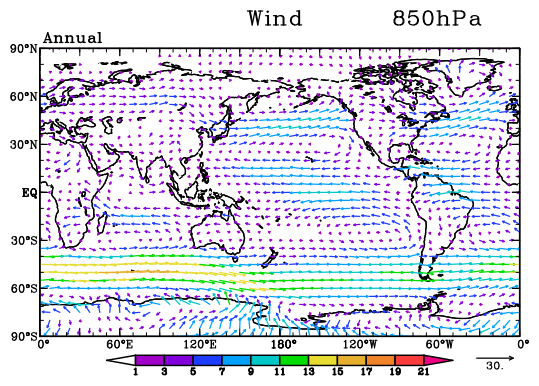
\includegraphics[width=0.85\textwidth]{images/ch03/p03_img01.png}
  \caption{Annual-mean wind field at 850\,hPa (vectors and isotachs, m\,s$^{-1}$). \hisu{열대: 무역풍 (NH 북동, SH 남동), 중위도: 편서풍 (SH에서 특히 강하고 대칭적, $\sim$15--21\,m\,s$^{-1}$), 아열대 고기압대: 약풍}}
  \label{fig:ch03-wind850}
\end{figure}

\begin{remark}[850\,hPa의 주요 특징]
\begin{itemize}
  \item \textgr{Trade winds}: NH에서 north-easterly, SH에서 south-easterly이며,
        subtropical high와 equatorial trough 사이의 pressure gradient에 의해 구동된다.
  \item \textgr{Midlatitude westerlies}: SH에서 특히 강하고 zonally symmetric하며
        ($\sim$15--21\,m\,s$^{-1}$), 이는 대규모 대륙의 부재를 반영한다.
  \item \textgr{Subtropical high belt}: Hadley cell이 하강하는 $30^{\circ}$\,N/S 부근에서
        wind speed가 약하다.
\end{itemize}
\end{remark}

\begin{hisublock}
850\,hPa 바람장에서 가장 눈에 띄는 것은 남반구 편서풍의 동서 대칭성이다.
대륙이 적어 지형 강제가 약하기 때문이다.
반면 북반구는 대륙과 해양의 비대칭 때문에 파동 구조가 뚜렷하다.
\end{hisublock}


\subsubsection{500\,hPa --- Mid-Troposphere}

\begin{figure}[ht]
  \centering
  % TODO: Extract figure from Ch03 lecture note, page 3
  % Description: Annual-mean 500 hPa wind field.  Flow is predominantly
  %   westerly at all latitudes outside the deep tropics.  SH flow is nearly
  %   zonally symmetric (20--30 m/s).  NH shows two jet maxima: one over
  %   East Asia and one over eastern North America.
  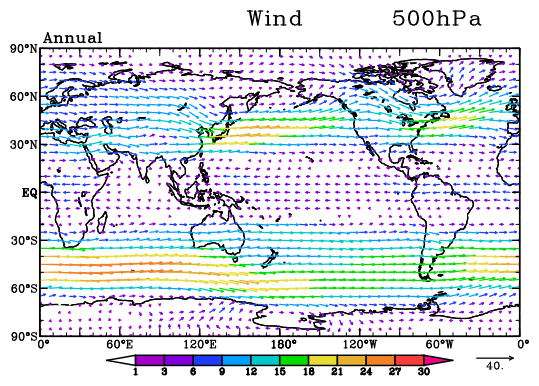
\includegraphics[width=0.85\textwidth]{images/ch03/p05_img01.png}
  \caption{Annual-mean wind field at 500\,hPa (vectors and isotachs, m\,s$^{-1}$). \hisu{열대 외 모든 위도에서 편서풍 우세; SH는 거의 동서 대칭 (20--30\,m\,s$^{-1}$); NH는 동아시아와 북미 동부에 두 개의 제트 극대}}
  \label{fig:ch03-wind500}
\end{figure}

\begin{remark}[500\,hPa의 주요 특징]
\begin{itemize}
  \item $\sim$$15^{\circ}$ 이상의 모든 위도에서 \textgr{westerly flow}가 우세하다.
  \item SH: 거의 zonally symmetric하며, wind speed 20--30\,m\,s$^{-1}$.
  \item NH: 두 개의 뚜렷한 jet maximum ---
        \begin{enumerate}
          \item East Asia ($\sim$$30^{\circ}$N, 130$^{\circ}$E)
          \item Eastern North America ($\sim$$40^{\circ}$N, 70$^{\circ}$W)
        \end{enumerate}
        이는 Himalaya--Tibet과 Rocky Mountain topography에 의한 stationary wave forcing을 반영한다.
\end{itemize}
\end{remark}

\hisu{500\,hPa는 대류권 중간으로, 지형에 의한 정상파(stationary wave)의 영향을 잘 보여준다.}


\subsubsection{200\,hPa --- Upper Troposphere}

\begin{figure}[ht]
  \centering
  % TODO: Extract figure from Ch03 lecture note, page 4
  % Description: Annual-mean 200 hPa wind field.  Subtropical jet streams are
  %   the dominant feature: East Asian jet exceeds 40 m/s, Atlantic jet is
  %   secondary.  SH subtropical jet is more continuous but weaker in amplitude.
  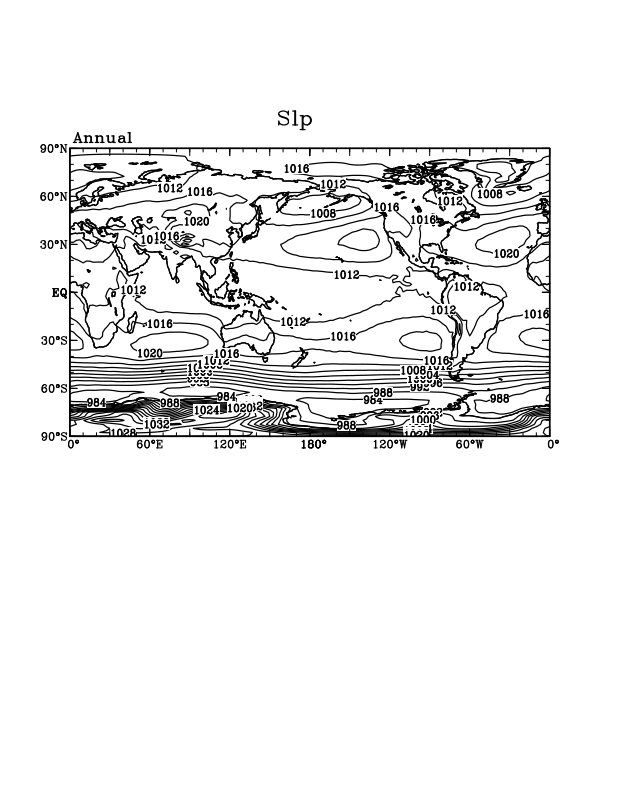
\includegraphics[width=0.85\textwidth]{images/ch03/p04_img01.png}
  \caption{Annual-mean wind field at 200\,hPa, highlighting the subtropical jet streams. \hisu{동아시아 제트가 최강 ($>$40\,m\,s$^{-1}$, 티벳 고원에 의해 고정), 대서양 제트는 이차 극대; SH 아열대 제트는 더 연속적이나 진폭은 약함}}
  \label{fig:ch03-wind200}
\end{figure}

\begin{remark}[200\,hPa의 주요 특징]
\begin{itemize}
  \item \textgr{Subtropical jet streams}이 $30^{\circ}$\,N/S 부근의 upper troposphere를 지배한다.
  \item East Asian jet: 연평균 기준 지구에서 가장 강하며, \textbf{40\,m\,s$^{-1}$}을 초과하고
        Tibetan Plateau에 의해 고정된다.
  \item Atlantic jet: North America 동부 해안 상공의 이차 극대이다.
  \item SH: subtropical jet이 더 연속적 (거의 circumpolar)이지만, 개별 극대의 진폭은
        NH보다 약하다.
\end{itemize}
\end{remark}

\begin{hisublock}
200\,hPa에서의 아열대 제트는 열대와 중위도 사이의 온도 경도에 의해 thermal wind
관계를 통해 설명된다 (Section~\ref{sec:ch03-thermal-wind}).
동아시아 제트가 특별히 강한 이유는 티벳 고원에 의한 diabatic heating과 정상파 강제
때문이다.
\end{hisublock}

\begin{hisublock}
\textbf{참고 문헌 가이드:}
\begin{itemize}
  \item Peixoto and Oort (1992), \textit{Physics of Climate}, Ch.7.4 (pp.149--161, 본 PDF에는 목차만 수록) -- mean circulation과 wind field의 전반적 관측 기술
  \item Hartmann (1994), \textit{Global Physical Climatology}, Ch.6.3 (pp.138--149, 본 PDF에는 목차만 수록) -- atmospheric motion과 meridional transport of energy
  \item Marshall and Plumb (2008), \textit{Atmosphere, Ocean and Climate Dynamics}, Ch.5.4 (pp.73--78, PDF pp.94--99) -- meridional structure of winds
\end{itemize}
\end{hisublock}


% ---------------------------------------------------------------------------------------
\subsection{Sea-Level Pressure}
% ---------------------------------------------------------------------------------------

\begin{figure}[ht]
  \centering
  % TODO: Extract figure from Ch03 lecture note, page 5--6
  % Description: Annual-mean sea-level pressure (SLP).  Subtropical highs
  %   (1016--1020 hPa) over all major ocean basins at ~30 deg.  Equatorial
  %   trough (1008--1012 hPa).  Subpolar lows: Aleutian Low, Icelandic Low
  %   (NH); deep circumpolar trough in SH (~984--988 hPa).
  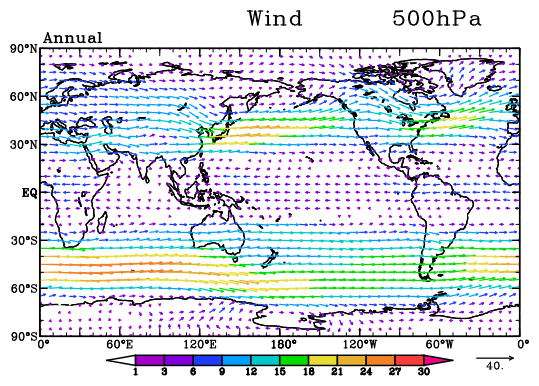
\includegraphics[width=0.85\textwidth]{images/ch03/p05_img01.png}
  \caption{Annual-mean sea-level pressure (hPa).  Contour interval: 4\,hPa. \hisu{아열대 고기압 ($\sim$1016--1020\,hPa, $\sim$$30^{\circ}$\,N/S 해양), 적도 기압골 ($\sim$1008--1012\,hPa), 아극 저기압 (Aleutian, Icelandic Low; SH 순환극 골 $\sim$984--988\,hPa)}}
  \label{fig:ch03-slp-ann}
\end{figure}

\begin{definition}[Major Pressure Centres]
The annual-mean SLP field is organised into a small number of recurring centres:
\begin{multicols}{2}
\textgr{Subtropical Highs} ($\sim$1016--1020\,hPa)\\
Located over each ocean basin near $30^{\circ}$\,N/S:
\begin{itemize}
  \item North Pacific High
  \item North Atlantic (Azores/Bermuda) High
  \item South Pacific High
  \item South Atlantic High
  \item South Indian Ocean High
\end{itemize}

\columnbreak

\textgr{Subpolar Lows}\\
\begin{itemize}
  \item Aleutian Low ($\sim$$50^{\circ}$N, 170$^{\circ}$W)
  \item Icelandic Low ($\sim$$62^{\circ}$N, 20$^{\circ}$W)
  \item SH circumpolar trough ($\sim$$65^{\circ}$S, $\sim$984--988\,hPa)
\end{itemize}
\vspace{4pt}
\textgr{Equatorial Trough}\\
$\sim$1008--1012\,hPa, slightly north of the equator in the annual mean.
\end{multicols}
\end{definition}

\begin{hisublock}
NH는 대륙--해양 대비가 크기 때문에 기압 분포가 비대칭적이다.
SH는 대륙이 적어 기압 패턴이 거의 동서 대칭이며, 특히 $65^{\circ}$S 부근의
순환극 저기압 골(circumpolar trough)은 매우 깊다.
\end{hisublock}

\begin{hisublock}
\textbf{참고 문헌 가이드:}
\begin{itemize}
  \item Peixoto and Oort (1992), \textit{Physics of Climate}, Ch.7.1 (pp.131--136, 본 PDF에는 목차만 수록) -- mass and pressure의 관측 분포
  \item Marshall and Plumb (2008), \textit{Atmosphere, Ocean and Climate Dynamics}, Ch.5.2 (pp.67--70, PDF pp.88--91) -- pressure and geopotential의 meridional structure
  \item Hartmann (1994), \textit{Global Physical Climatology}, Ch.6.5 (pp.155--169, 본 PDF에는 목차만 수록) -- large-scale circulation pattern과 주요 기압 중심
\end{itemize}
\end{hisublock}


% ---------------------------------------------------------------------------------------
\subsection{Zonal Mean vs.\ Eddy Decomposition}
\label{sec:ch03-eddy-decomp}
% ---------------------------------------------------------------------------------------

임의의 atmospheric field $A(\lambda, \phi, p, t)$는 다음과 같이 분해할 수 있다:
\begin{equation}
  A = [A] + A^{*},
\end{equation}
여기서 $[A]$는 zonal mean이고 $A^{*} \equiv A - [A]$는 \textgr{eddy} (zonal mean으로부터의 편차)이다.

\subsubsection{Zonal-Mean Zonal Wind}

\begin{figure}[ht]
  \centering
  % TODO: Extract figure from Ch03 lecture note, page 8
  % Description: Latitude--pressure cross-section of annual-mean zonal-mean
  %   zonal wind [u].  Two westerly maxima at ~200 hPa near 30N and 30S
  %   (subtropical jets, ~30 m/s).  Weak easterlies in the deep tropics
  %   and near the surface at high latitudes.
  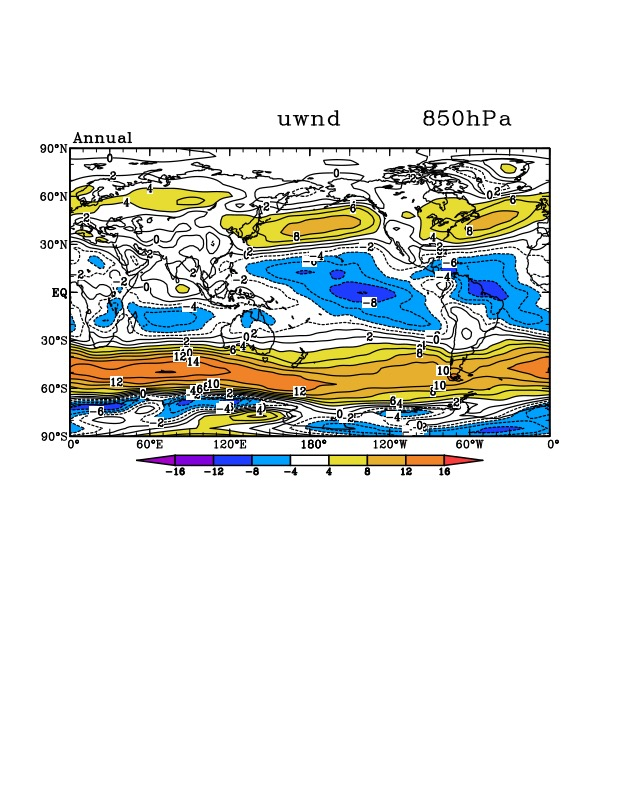
\includegraphics[width=0.85\textwidth]{images/ch03/p08_img01.jpeg}
  \caption{Annual-mean $[\bar{u}]$ (m\,s$^{-1}$), latitude--pressure cross-section. \hisu{$\sim$200\,hPa, $30^{\circ}$N/S 부근에 아열대 제트 ($\sim$30\,m\,s$^{-1}$); 열대 대류권 전체에 약한 동풍; 지표에서 $\sim$$30^{\circ}$ 경계로 저위도 동풍(무역풍)과 고위도 서풍}}
  \label{fig:ch03-zmzw}
\end{figure}

\begin{remark}[Zonal-mean zonal wind 구조]
\begin{itemize}
  \item $\sim$200\,hPa, $30^{\circ}$N 및 $30^{\circ}$S 부근에 두 개의 \textgr{westerly jet maximum}이 존재하며,
        연평균 peak speed는 $\sim$30\,m\,s$^{-1}$이다.
  \item 대류권 전체에 걸쳐 약한 tropical easterlies가 나타난다.
  \item $\sim$$30^{\circ}$ 저위도 쪽에는 surface easterlies (trades),
        $\sim$$30^{\circ}$ 고위도 쪽에는 surface westerlies가 분포한다.
\end{itemize}
\end{remark}


\subsubsection{Zonal-Mean Meridional Wind}

\begin{figure}[ht]
  \centering
  % TODO: Extract figure from Ch03 lecture note, page 9
  % Description: Latitude--pressure cross-section of [v].  Very small values
  %   (~0.3 m/s), but a clear Hadley cell signal: poleward flow at upper
  %   levels, equatorward flow at low levels in the tropics.
  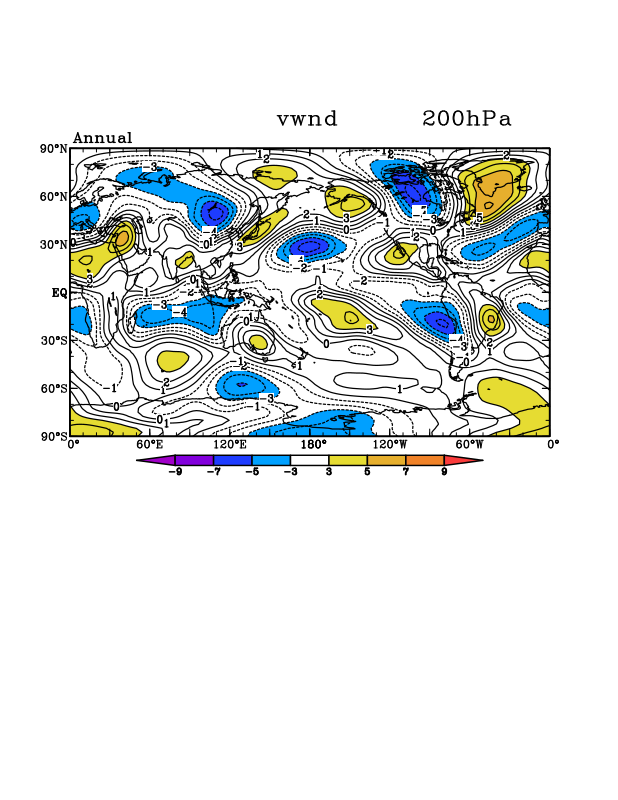
\includegraphics[width=0.85\textwidth]{images/ch03/p09_img01.png}
  \caption{Annual-mean $[\bar{v}]$ (m\,s$^{-1}$).  Note the much smaller contour interval
           compared to $[\bar{u}]$. \hisu{값이 매우 작지만 ($\sim$0.3\,m\,s$^{-1}$) 해들리 셀 신호가 명확: 상층 극방향 흐름, 하층 적도방향 흐름}}
  \label{fig:ch03-zmvw}
\end{figure}

\hisu{$[\bar{v}]$는 $[\bar{u}]$에 비해 한 자릿수 이상 작지만,
해들리 셀을 통한 질량 수송을 반영하는 중요한 양이다.}


\subsubsection{Geopotential Height: Full Field and Eddy Field}

\begin{figure}[ht]
  \centering
  % TODO: Extract figure from Ch03 lecture note, pages 10--12
  % Description: Geopotential height maps at 200, 500, and 850 hPa --- both
  %   full field and eddy (Z*) field.  NH eddy field shows wave-2 to wave-3
  %   pattern (troughs over eastern North America and East Asia); SH eddy
  %   amplitudes are much weaker.
  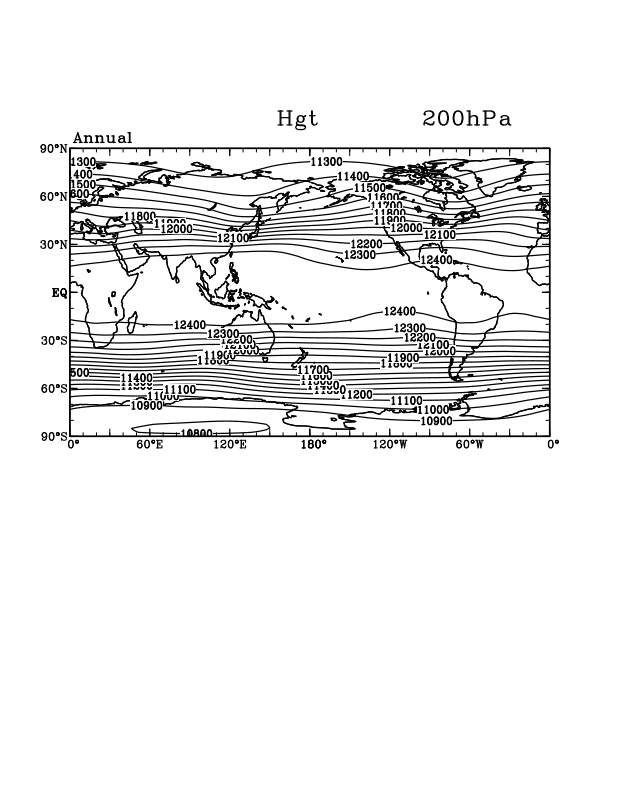
\includegraphics[width=0.5\textwidth]{images/ch03/p10_img01.png}
  \caption{Annual-mean geopotential height at 500\,hPa: (a)~full field, (b)~eddy field $Z^{*}$. \hisu{NH $Z^{*}$: wave-2$\sim$3 패턴 (북미 동부, 동아시아 상공 기압골); SH: eddy 진폭이 훨씬 약함 --- 지형 강제 부재 반영}}
  \label{fig:ch03-z500-eddy}
\end{figure}

\begin{remark}[Eddy geopotential height]
\begin{itemize}
  \item NH: eddy field $Z^{*}$는 500\,hPa에서 뚜렷한 \textbf{wave-2$\sim$wave-3 pattern}을 보이며,
        eastern North America와 East Asia 상공에 trough, eastern ocean basin 상공에 ridge가 위치한다.
  \item SH: eddy 진폭이 훨씬 약하며, 이는 SH circulation의 zonally symmetric한 성격과
        topographic forcing의 상대적 부재를 반영한다.
  \item Eddy 진폭은 일반적으로 고도에 따라 증가 (850\,hPa보다 200\,hPa에서 더 큼)하며,
        이는 stationary Rossby wave의 equivalent-barotropic structure와 일치한다.
\end{itemize}
\end{remark}

\begin{hisublock}
eddy($A^{*}$)는 동서 평균에서 벗어난 파동 구조를 의미한다.
NH에서는 대륙--해양 대비와 대규모 지형(히말라야, 로키) 때문에 eddy 진폭이 크고,
SH에서는 작다. 이것이 NH 기후의 ``비대칭성''의 핵심이다.
\end{hisublock}

\begin{hisublock}
\textbf{참고 문헌 가이드:}
\begin{itemize}
  \item Peixoto and Oort (1992), \textit{Physics of Climate}, Ch.7.3 (pp.144--148, 본 PDF에는 목차만 수록) -- geopotential height의 관측 분포 및 eddy 분해
  \item Hartmann (1994), \textit{Global Physical Climatology}, Ch.6.3 (pp.138--149, 본 PDF에는 목차만 수록) -- zonal mean wind와 eddy 구조
  \item Marshall and Plumb (2008), \textit{Atmosphere, Ocean and Climate Dynamics}, Ch.8.1 (pp.140--141, PDF pp.161--162) -- understanding the observed circulation
\end{itemize}
\end{hisublock}


\subsubsection{Eddy Variance: $\overline{v_{E}^{2}}$ and $\overline{u_{E}^{2}}$}
\label{sec:ch03-eddy-variance}

Eddy component의 운동 에너지 분포를 이해하기 위해 $\overline{v_{E}^{2}}$와 $\overline{u_{E}^{2}}$의
위도별 구조를 분석할 수 있다.  여기서 overline은 zonal average를 나타내고,
$u_{E} = u - [u]$, $v_{E} = v - [v]$는 eddy wind component이다.

\begin{definition}[Eddy Variance from an Idealized Stationary Wave]
Equator와 Pole 사이에서 streamfunction이 다음과 같이 단일 극대의 진폭 분포를 갖는
이상화된 정상파를 고려하자:
\begin{equation}
  \psi(\lambda, \phi) = A(\phi)\,\cos(k\lambda),
  \label{eq:idealized-wave}
\end{equation}
여기서 $A(\phi)$는 $\phi = \phi_{B}$ (적도와 극 사이 중간 위도)에서 단일 극대를 갖고,
$\phi = \phi_{A}$ (적도 측)과 $\phi = \phi_{C}$ (극 측)에서는 0에 가까운 bell-shaped function이다.
\end{definition}

\begin{remark}[Eddy wind component의 유도]
Geostrophic relation에 의해 eddy wind는 streamfunction으로부터 다음과 같이 얻어진다:
\begin{align}
  v_{E} &\propto \frac{\partial \psi}{\partial x}
         \propto -A(\phi)\,\sin(k\lambda),
  \label{eq:vE-from-psi} \\
  u_{E} &\propto -\frac{\partial \psi}{\partial y}
         \propto -\frac{dA}{d\phi}\,\cos(k\lambda).
  \label{eq:uE-from-psi}
\end{align}
\end{remark}

\begin{theorem}[Zonal-Mean Eddy Variance의 위도 구조]
\label{thm:eddy-variance}
이상화된 정상파 \eqref{eq:idealized-wave}로부터 zonal-mean eddy variance는 다음과 같다:
\begin{align}
  \overline{v_{E}^{2}} &\propto A(\phi)^{2},
  \label{eq:vE2-structure} \\
  \overline{u_{E}^{2}} &\propto \left(\frac{dA}{d\phi}\right)^{2}.
  \label{eq:uE2-structure}
\end{align}
\end{theorem}

\begin{proof}
Zonal average ($\lambda$ 방향 적분)에서
$\overline{\sin^{2}(k\lambda)} = \overline{\cos^{2}(k\lambda)} = \frac{1}{2}$이므로,
식~\eqref{eq:vE-from-psi}과 \eqref{eq:uE-from-psi}를 제곱하고 zonal average를 취하면:
\[
  \overline{v_{E}^{2}} \propto A(\phi)^{2}\,\overline{\sin^{2}(k\lambda)}
                        = \tfrac{1}{2}\,A(\phi)^{2},
\]
\[
  \overline{u_{E}^{2}} \propto \left(\frac{dA}{d\phi}\right)^{2}\,\overline{\cos^{2}(k\lambda)}
                        = \tfrac{1}{2}\,\left(\frac{dA}{d\phi}\right)^{2}.
\]
$A(\phi)$가 $\phi_{B}$에서 \textbf{단일 극대}를 가지므로,
$A(\phi)^{2}$ 역시 $\phi_{B}$에서 단일 극대를 갖는다 $\Rightarrow$ $\overline{v_{E}^{2}}$는 \textbf{단일 극대}.

반면 $dA/d\phi$는 $\phi_{B}$에서 0이 되고 (극대에서 기울기 = 0),
$\phi_{A}$ 쪽에서 양, $\phi_{C}$ 쪽에서 음이므로,
$(dA/d\phi)^{2}$는 $\phi_{B}$ 양쪽에 \textbf{두 개의 극대}를 갖는다
$\Rightarrow$ $\overline{u_{E}^{2}}$는 \textbf{한 쌍의 극대}.
\end{proof}

\begin{hisublock}
물리적 해석:
\begin{itemize}
  \item \textbf{$\overline{v_{E}^{2}}$가 단일 극대}: 파동 진폭이 최대인 위도 $\phi_{B}$에서
        streamline의 \textbf{남북 방향 진동}이 가장 크다.
        이곳에서 $v_{E}$ (남북풍 섭동)가 최대이므로 $\overline{v_{E}^{2}}$도 여기서 극대.
  \item \textbf{$\overline{u_{E}^{2}}$가 두 개의 극대}: 파동 진폭의 \textbf{위도별 기울기}가 최대인 곳
        ($\phi_{A}$, $\phi_{C}$)에서 streamline이 동서 방향으로 가장 많이 압축/신장된다.
        연속 방정식 $\partial u_{E}/\partial x + \partial v_{E}/\partial y = 0$에 의해,
        남북풍 $v_{E}$의 위도 변화가 동서풍 섭동 $u_{E}$를 유발하기 때문이다.
        파동 진폭 중심($\phi_{B}$)에서는 $dA/d\phi = 0$이므로 $u_{E} \approx 0$.
\end{itemize}
\end{hisublock}

\begin{hisublock}
HW 문제에서 주어진 이상화된 파동 그림의 핵심 포인트:
\begin{itemize}
  \item 위도 B (중간): streamline이 가장 크게 남북으로 사행 $\Rightarrow$ $v_{E}$ 최대 $\Rightarrow$ $\overline{v_{E}^{2}}$ 단일 극대
  \item 위도 A, C (양 측면): streamline이 zonal 방향으로 모이거나 벌어짐 $\Rightarrow$ $u_{E}$ 최대 $\Rightarrow$ $\overline{u_{E}^{2}}$ 한 쌍의 극대
  \item 수학적으로: $\overline{v_{E}^{2}} \propto A^{2}$ (단일 극대), $\overline{u_{E}^{2}} \propto (dA/d\phi)^{2}$ (쌍 극대)
\end{itemize}
\end{hisublock}

\begin{hisublock}
\textbf{참고 문헌 가이드:}
\begin{itemize}
  \item Holton (2012), \textit{An Introduction to Dynamic Meteorology}, Ch.5.7 (pp.127--140) -- plane wave kinematics와 eddy wind component의 유도
  \item Peixoto and Oort (1992), \textit{Physics of Climate}, Ch.7.3 (pp.144--148) -- eddy kinetic energy의 관측 분포
  \item Lorenz (1967), \textit{The Nature and Theory of the General Circulation of the Atmosphere} -- eddy energy budget의 기초 이론
\end{itemize}
\end{hisublock}


% ---------------------------------------------------------------------------------------
\subsection{Thermal Wind and Jet Streams}
\label{sec:ch03-thermal-wind}
% ---------------------------------------------------------------------------------------

Geostrophic wind의 vertical shear는 horizontal temperature gradient와 \textgr{thermal wind relation}을 통해 연결된다:
\begin{equation}
  \frac{\partial u_g}{\partial \ln p} = \frac{R}{f}\,\frac{\partial T}{\partial y},
  \label{eq:thermal-wind-ch03}
\end{equation}
여기서 $R$은 dry air의 gas constant이고 $f$는 Coriolis parameter이다.
NH에서 meridional temperature gradient $\partial T/\partial y < 0$ (온도가 극 방향으로 감소)이므로,
westerly wind는 고도에 따라 \emph{증가}하여 $\sim$200\,hPa에서 subtropical jet을 형성한다.

\begin{figure}[ht]
  \centering
  % TODO: Extract figure from Ch03 lecture note, page 13
  % Description: Side-by-side latitude--pressure cross-sections of (a) zonal-mean
  %   temperature [T] and (b) zonal-mean zonal wind [u], illustrating the thermal
  %   wind relationship: steepest temperature gradients correspond to strongest
  %   vertical wind shear and jet maxima at ~200 hPa.
  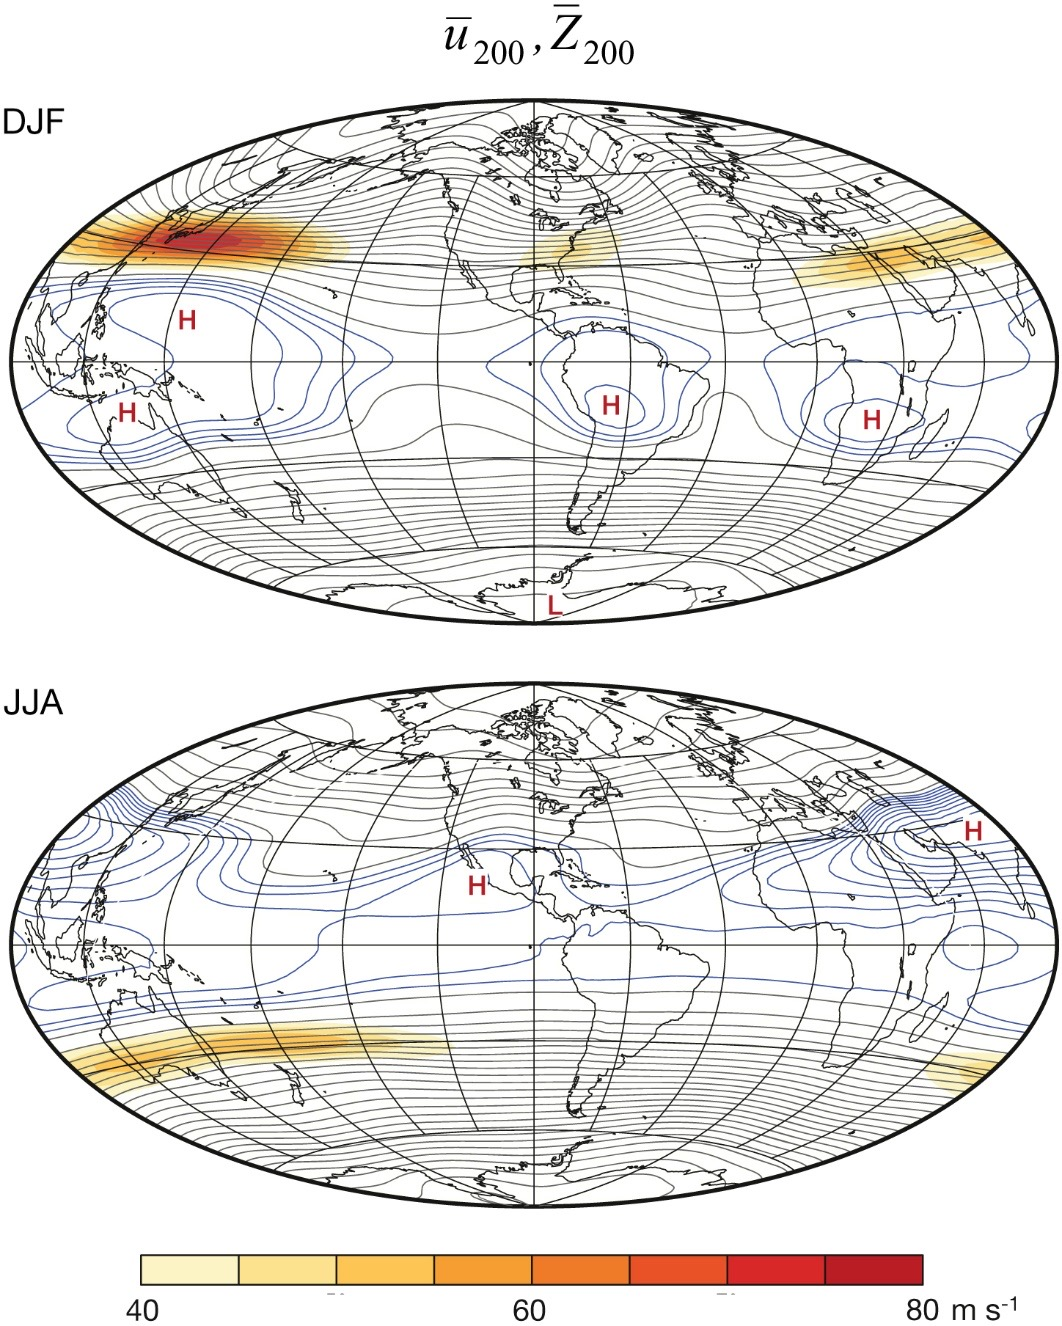
\includegraphics[width=0.5\textwidth]{images/ch03/p13_img01.jpeg}
  \caption{Annual-mean (a) $[\bar{T}]$ (K) and (b) $[\bar{u}]$ (m\,s$^{-1}$),
           illustrating the thermal wind relationship. \hisu{가장 급한 남북 $T$ 경도가 가장 강한 연직 바람 시어 및 $\sim$200\,hPa 제트 극대에 대응}}
  \label{fig:ch03-thermal-wind}
\end{figure}

\begin{example}[Thermal wind estimate of the subtropical jet]
Take a meridional temperature gradient $\Delta T / \Delta y \approx -15$\,K over
$20^{\circ}$ latitude ($\sim$2200\,km) between $15^{\circ}$N and $35^{\circ}$N.  Then the
thermal wind shear from 850\,hPa to 200\,hPa ($\Delta \ln p \approx 1.45$) gives:
\[
  \Delta u \approx \frac{R}{f}\,\frac{\Delta T}{\Delta y}\,\Delta \ln p
           \approx \frac{287}{7.3\times10^{-5}}\,\frac{15}{2.2\times10^{6}}\,1.45
           \approx 39\;\text{m\,s}^{-1}.
\]
This is consistent with the observed subtropical jet speed of $\sim$40\,m\,s$^{-1}$.
\end{example}

\hisu{thermal wind: 남북 온도 경도가 클수록 연직 바람 시어가 강해지고,
상층 제트가 강해진다. 이것이 아열대 제트의 핵심 메커니즘이다.}

\begin{hisublock}
\textbf{참고 문헌 가이드:}
\begin{itemize}
  \item Holton (2012), \textit{An Introduction to Dynamic Meteorology}, Ch.10.2 -- thermal wind과 jet stream의 이론적 기초
  \item Hartmann (1994), \textit{Global Physical Climatology}, Ch.6.3 (pp.138--149, 본 PDF에는 목차만 수록) -- atmospheric motion과 meridional transport
  \item Peixoto and Oort (1992), \textit{Physics of Climate}, Ch.7.4 (pp.149--161, 본 PDF에는 목차만 수록) -- mean circulation에서의 jet stream 관측
\end{itemize}
\end{hisublock}


% ---------------------------------------------------------------------------------------
\subsection{Meridional Overturning Circulation}
\label{sec:ch03-hadley}
% ---------------------------------------------------------------------------------------

\begin{figure}[ht]
  \centering
  % TODO: Extract figure from Ch03 lecture note, page 14--15
  % Description: (a) Zonal-mean omega (Pa/s) cross-section: negative omega
  %   (ascent) centred on the equator, positive omega (descent) in subtropics.
  %   (b) Zonal-mean meridional wind [v]: low-level convergence toward
  %   equator, upper-level divergence poleward --- the Hadley cell signature.
  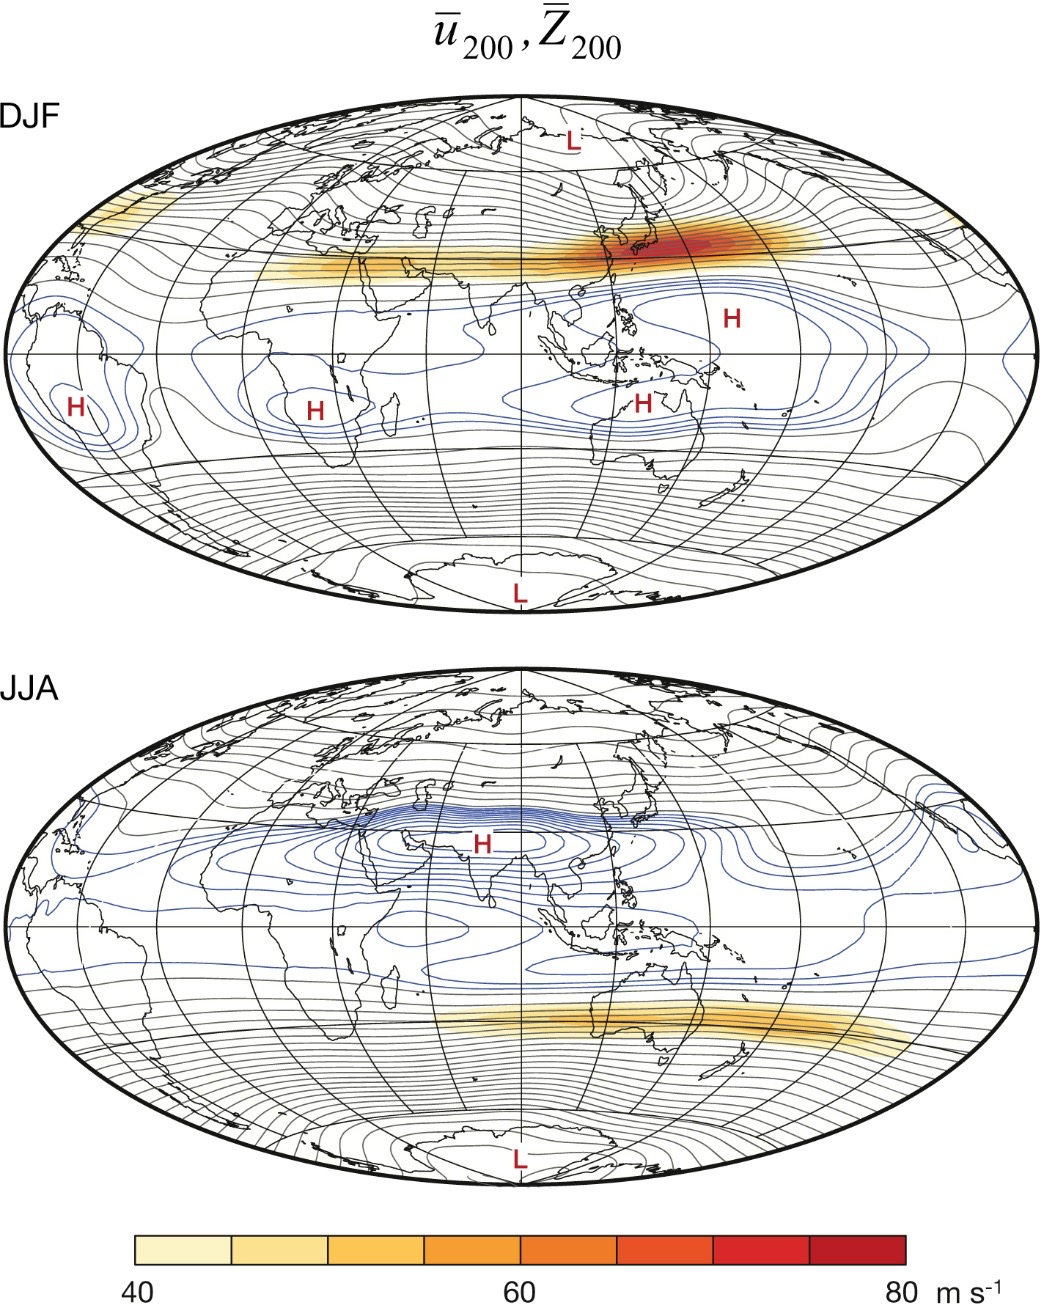
\includegraphics[width=0.85\textwidth]{images/ch03/p14_img01.jpeg}
  \caption{Annual-mean (a) $[\bar{\omega}]$ (Pa\,s$^{-1}$) and
           (b) $[\bar{v}]$ (m\,s$^{-1}$), showing the Hadley cell structure. \hisu{$\omega<0$ (상승)은 적도 중심, $\omega>0$ (하강)은 아열대; $[\bar{v}]$: 하층 적도 수렴, 상층 극방향 발산}}
  \label{fig:ch03-hadley-ann}
\end{figure}

\begin{definition}[Hadley Cell --- Annual Mean]
The annual-mean Hadley cell is characterised by:
\begin{itemize}
  \item \textgr{Ascending motion} at the equator ($[\bar{\omega}] < 0$): deep convection in the ITCZ
        releases latent heat and drives upward mass flux.
  \item \textgr{Poleward flow} in the upper troposphere ($\sim$200\,hPa): $[\bar{v}] > 0$ in the NH,
        $[\bar{v}] < 0$ in the SH.
  \item \textgr{Descending motion} in the subtropics ($\sim$$30^{\circ}$\,N/S, $[\bar{\omega}] > 0$):
        adiabatic warming maintains the subtropical highs and suppresses precipitation.
  \item \textgr{Equatorward return flow} at the surface: the trade winds.
\end{itemize}
\end{definition}

\begin{hisublock}
적도에서 상승, 아열대에서 하강 --- 이것이 해들리 셀의 기본 구조이다.
연평균에서는 NH 셀과 SH 셀이 거의 대칭이지만, 계절적으로는 겨울 반구 셀이
훨씬 강해지고 적도를 넘어 확장한다 (Section~\ref{sec:ch03-seasonal}).
\end{hisublock}

\begin{hisublock}
\textbf{참고 문헌 가이드:}
\begin{itemize}
  \item Hartmann (1994), \textit{Global Physical Climatology}, Ch.6.3 (pp.138--149, 본 PDF에는 목차만 수록) -- Hadley cell과 meridional overturning의 관측
  \item Peixoto and Oort (1992), \textit{Physics of Climate}, Ch.7.4 (pp.149--161, 본 PDF에는 목차만 수록) -- mean meridional circulation의 상세 관측
  \item Marshall and Plumb (2008), \textit{Atmosphere, Ocean and Climate Dynamics}, Ch.5.4 (pp.73--78, PDF pp.94--99) -- meridional overturning circulation (Fig.~5.21, p.76, PDF p.97)
\end{itemize}
\end{hisublock}


% ---------------------------------------------------------------------------------------
\subsection{Stationary Wave Patterns}
% ---------------------------------------------------------------------------------------

Circulation의 zonally asymmetric 성분 (stationary waves)은 다음 두 가지 원인에서 발생한다:
\begin{itemize}
\item \textgr{Orographic forcing}: 대규모 산맥 (Rockies, Himalayas/Tibet) 위를 지나는 흐름
\item \textgr{Thermal forcing}: land--sea heating contrast와 SST gradient
\end{itemize}

\begin{remark}[Cross-Equatorial Stationary Wave Response]
Solstitial season에 한쪽 반구에 국한된 비대칭 thermal forcing에도 불구하고, stationary wave response는 적도에 대해 거의 대칭일 수 있다. 두 가지 메커니즘이 이를 설명한다:
\begin{enumerate}
\item \textgr{Rossby wave source}: tropical heating에 의한 upper-level divergence가 Rossby wave source를 생성하고, waveguide effect를 통해 양쪽 반구로 전파된다.
\item \textgr{Cross-equatorial mean flow}: Hadley cell의 강한 upper-level cross-equatorial flow가 waveguide 역할을 하여 wave activity를 적도 너머로 전달한다 (Hoskins and Karoly, 1981).
\end{enumerate}
\end{remark}
\begin{hisublock}
열대 가열이 한쪽 반구에만 있어도 정상파 응답이 적도 대칭일 수 있다:
(1) 로스비 파원이 양쪽 반구로 전파, (2) 해들리 셀의 적도 횡단 흐름이 파동 도파관 역할.
Ref: (Hoskins and Karoly, 1981)
\end{hisublock}

\begin{hisublock}
\textbf{참고 문헌 가이드:}
\begin{itemize}
  \item Hartmann (1994), \textit{Global Physical Climatology}, Ch.6.5 (pp.155--169, 본 PDF에는 목차만 수록) -- stationary wave, monsoon, Walker circulation 등 large-scale circulation pattern
  \item Held et al.\ (2002), ``Northern winter stationary waves: Theory and modeling'' -- stationary wave의 orographic/thermal forcing 이론
  \item Hoskins and Karoly (1981), ``The steady linear response of a spherical atmosphere to thermal and orographic forcing'' -- cross-equatorial wave response의 기초 이론
\end{itemize}
\end{hisublock}


\subsubsection{Seasonal Comparison of Stationary Wave Amplitude}

\begin{figure}[ht]
  \centering
  % TODO: Extract figure from Ch03 lecture note, page 13--14
  % Description: Z(200hPa) and u(200hPa) maps for DJF and JJA from Wallace et al.
  %   DJF NH: very pronounced wave-2 to wave-3 pattern with deep troughs over
  %   eastern N. America and East Asia, ridges over eastern Pacific and Atlantic.
  %   JJA NH: stationary wave pattern much weaker, nearly zonal.
  %   SH: weak stationary waves in both seasons.
  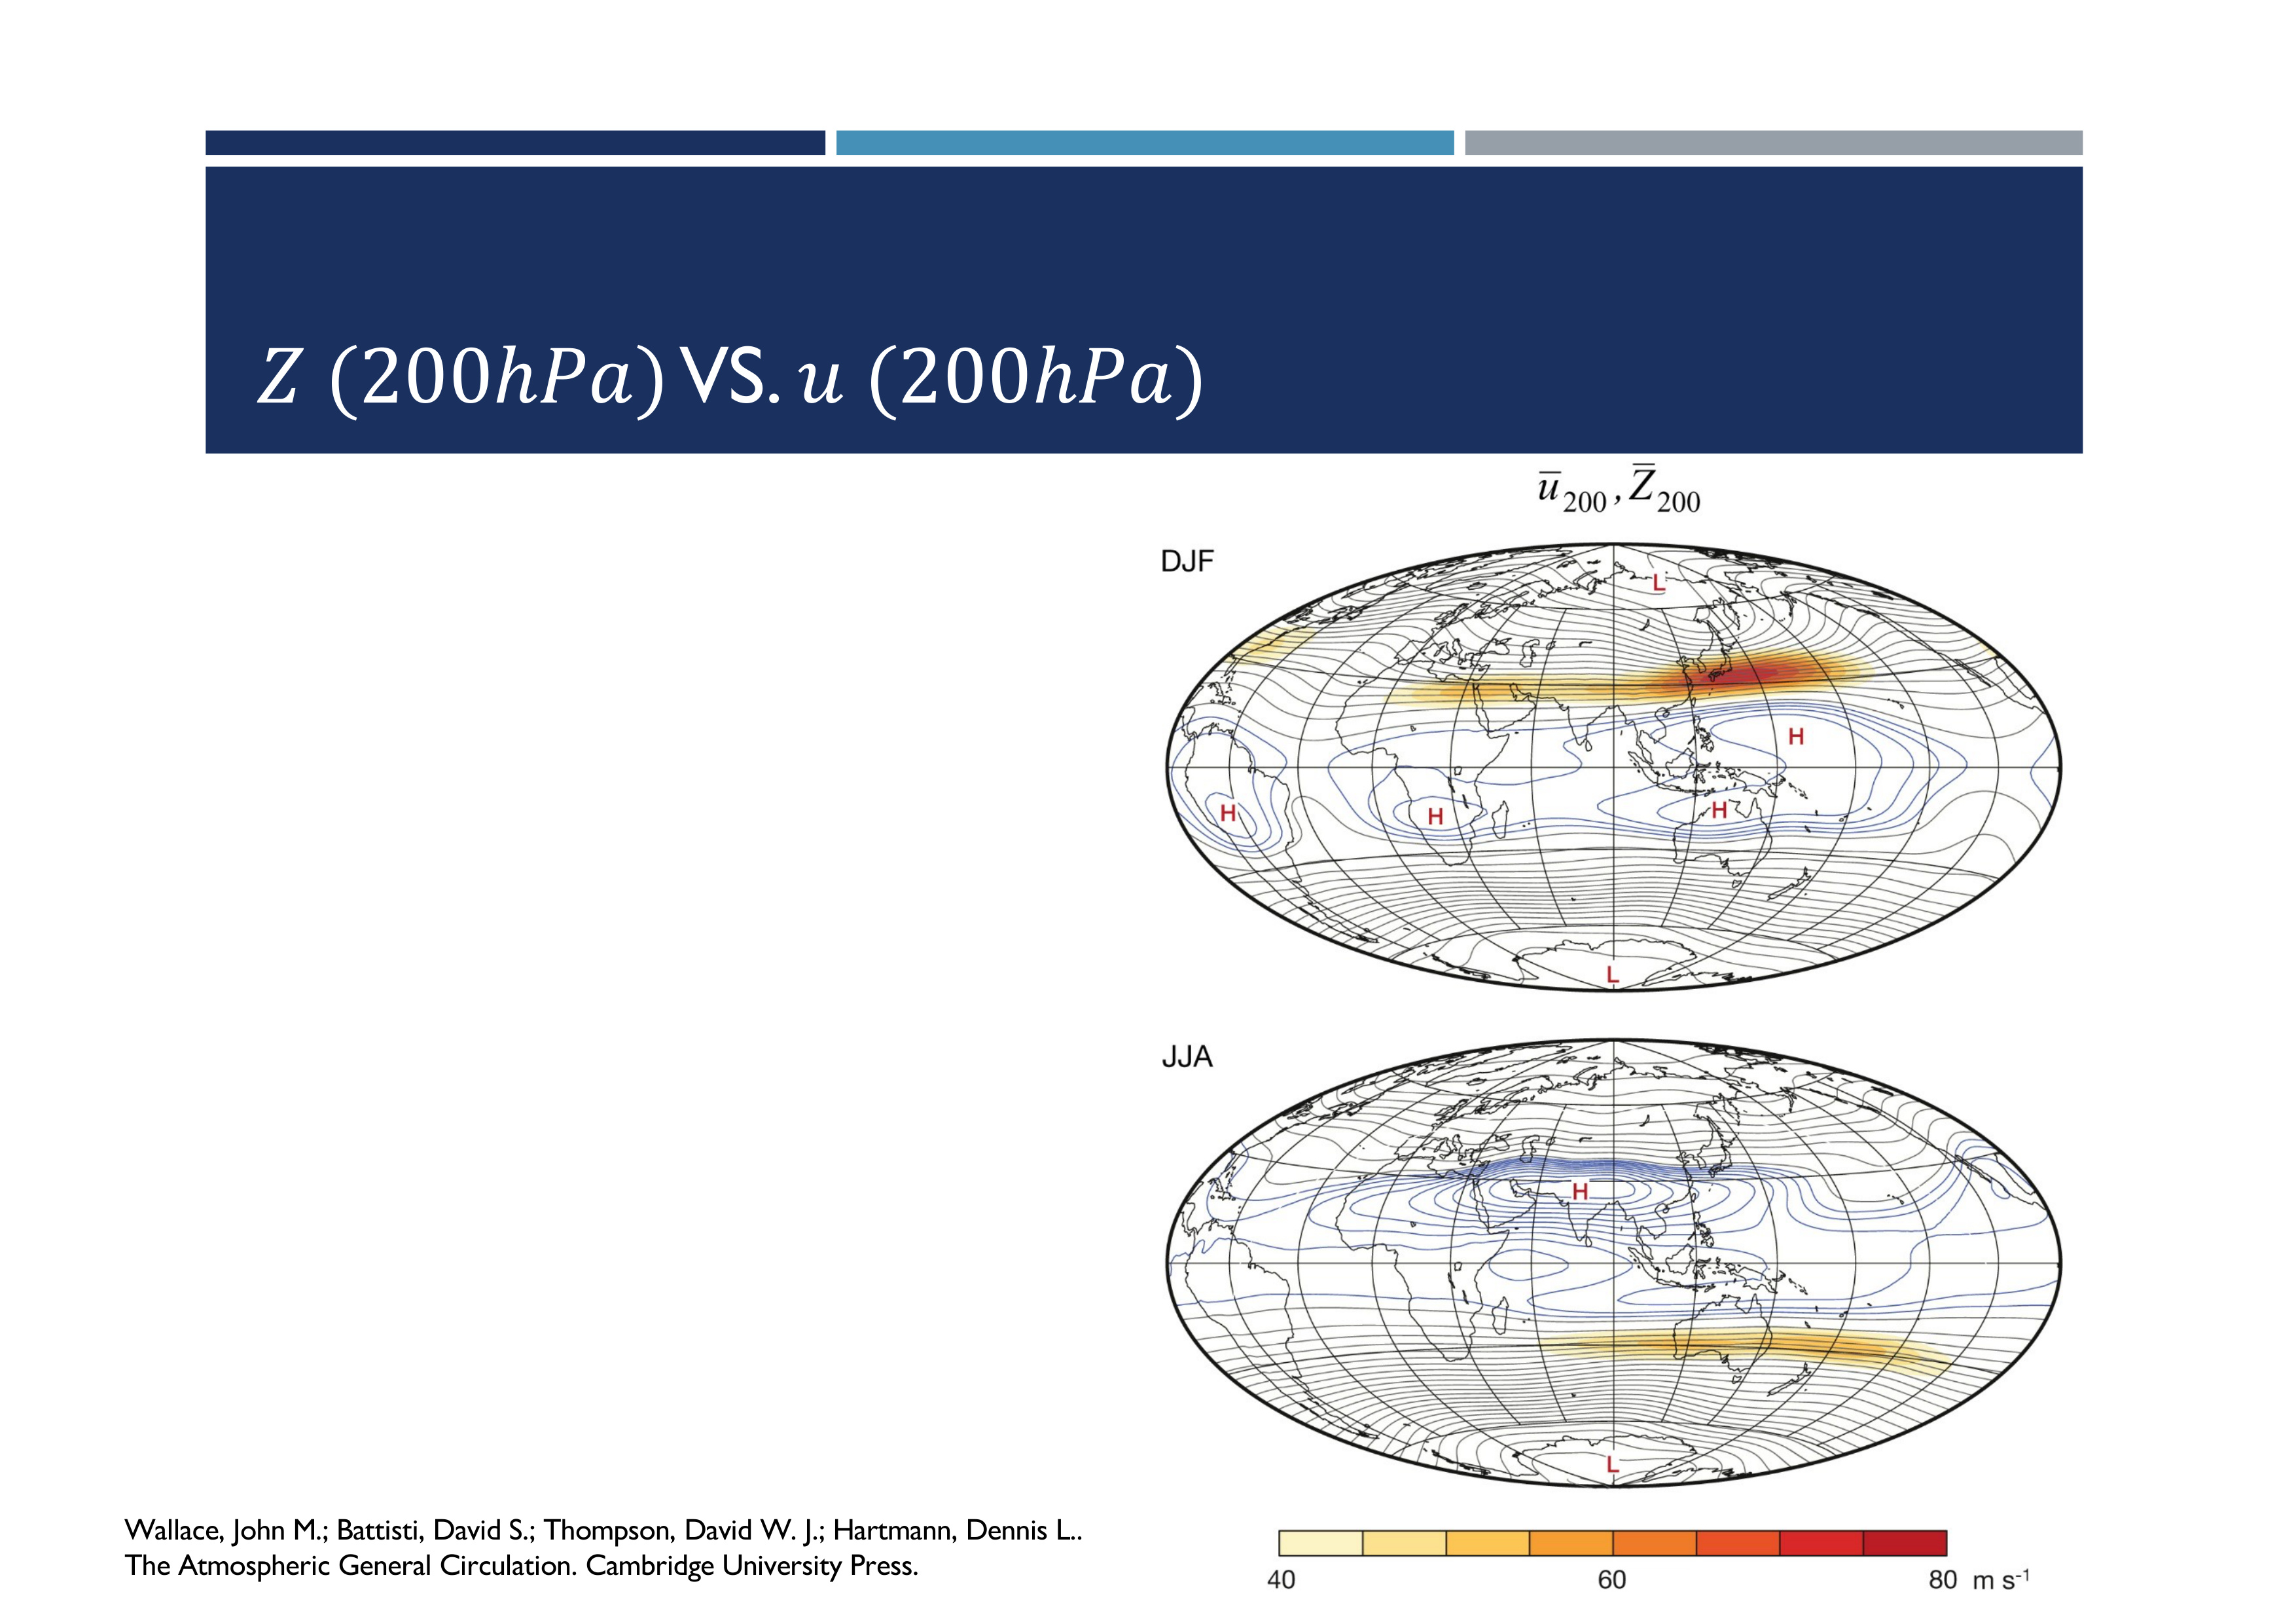
\includegraphics[width=0.85\textwidth]{images/ch03/p13_img02.jpeg}
  \caption{Climatological 200\,hPa geopotential height $\bar{Z}_{200}$ and zonal wind
           $\bar{u}_{200}$ (m\,s$^{-1}$, shading) for DJF (top) and JJA (bottom).
           \hisu{DJF NH: 뚜렷한 wave-2$\sim$3 패턴 (동아시아/북미 동부 기압골, 동태평양/대서양 기압능);
                  JJA NH: 정상파 크게 약화, 거의 동서 대칭;
                  SH: 양 계절 모두 약한 정상파}}
  \label{fig:ch03-z200-seasonal-stationary}
\end{figure}

200\,hPa geopotential height field에서 정상파의 계절별 진폭 차이는 극적이다.

\begin{definition}[Stationary Wave Amplitude --- Winter vs.\ Summer]
\textgr{Winter hemisphere} (DJF for NH, JJA for SH)의 upper tropospheric stationary wave는
\textgr{summer hemisphere}보다 \textbf{훨씬 큰 진폭}을 보인다.
\begin{multicols}{2}
\textgr{DJF (NH winter):}
\begin{itemize}
  \item 200\,hPa $Z^{*}$ eddy 진폭: $\sim$90--120\,m
  \item 뚜렷한 wave-2$\sim$wave-3 pattern: eastern N.\ America와 East Asia 상공에 deep trough, eastern ocean basins 상공에 ridge
  \item 국지 jet speed $>$50\,m\,s$^{-1}$ (East Asian jet)
  \item 수 개의 high (H) / low (L) 중심이 명확하게 식별 가능
\end{itemize}

\columnbreak

\textgr{JJA (NH summer):}
\begin{itemize}
  \item 200\,hPa $Z^{*}$ eddy 진폭: $\sim$30--50\,m (겨울의 $\sim$1/3)
  \item 흐름이 거의 \textbf{zonally symmetric}하여 stationary wave 구조가 약함
  \item Tibetan High가 유일한 뚜렷한 anticyclonic 편차
  \item Jet speed도 크게 약화
\end{itemize}
\end{multicols}
SH에서는 양 계절 모두 stationary wave 진폭이 NH 겨울의 $\sim$1/3 이하이며,
이는 topographic forcing이 약한 것을 반영한다.
\end{definition}

\begin{remark}[Winter stationary wave가 강한 이유]
겨울 반구에서 정상파 진폭이 강한 이유는 세 가지로 요약된다:
\begin{enumerate}
  \item \textgr{Stronger baroclinicity}: 겨울에 적도--극 온도 경도가 최대이므로 thermal wind에 의한
        평균 서풍류 $\bar{u}$가 강하고, Rossby wave의 전파 조건이 유리하다.
        정상 Rossby wave의 meridional wave number는 $l^{2} = \beta/\bar{u} - k^{2}$이므로,
        적절한 강도의 서풍($\bar{u}$)이 정상파 전파를 허용한다.
  \item \textgr{Stronger land--sea heating contrast}: 겨울 대륙은 급격히 냉각되어
        thermal forcing에 의한 정상파 강제가 여름보다 크다.
  \item \textgr{More effective waveguide}: 강한 겨울 제트 스트림은 정상 Rossby wave의
        meridional waveguide 역할을 하여, 파동 에너지를 효과적으로 가두고 증폭시킨다.
\end{enumerate}
여름에는 이 세 요인이 모두 약화되어, stationary wave 진폭이 겨울의 $\sim$1/3 수준으로 감소한다.
\end{remark}

\begin{hisublock}
겨울 반구에서 정상파가 강한 이유의 핵심: (1) 온도 경도 최대 $\rightarrow$ 서풍 최대 $\rightarrow$ 파동 전파 유리,
(2) 대륙 냉각으로 land--sea 열적 대비 극대, (3) 강한 제트가 도파관 역할.
HW 문제 포인트: DJF NH $Z^{*}_{200}$에서 wave-2$\sim$3이 뚜렷하지만,
JJA NH에서는 거의 동서 대칭. SH는 항상 약함 (대륙이 적어 지형/열적 강제 모두 약함).
\end{hisublock}

\begin{hisublock}
\textbf{참고 문헌 가이드:}
\begin{itemize}
  \item Holton (2012), \textit{An Introduction to Dynamic Meteorology}, Ch.10.5 -- stationary Rossby wave의 전파 조건과 $l^{2} = \beta/\bar{u} - k^{2}$
  \item Held et al.\ (2002), ``Northern winter stationary waves: Theory and modeling'' -- 겨울 정상파의 orographic/thermal forcing 분석
  \item Wallace, Battisti, Thompson, Hartmann, \textit{The Atmospheric General Circulation}, Ch.3 -- 200\,hPa $Z$ 및 $u$의 DJF/JJA 비교 그림
\end{itemize}
\end{hisublock}


% =======================================================================================
\section{Seasonal Variation}
\label{sec:ch03-seasonal}
% =======================================================================================

\subsection{Sea-Level Pressure}

\begin{figure}[ht]
  \centering
  % TODO: Extract figure from Ch03 lecture note, page 17--18
  % Description: SLP maps for DJF and JJA.  DJF: deep Aleutian Low and Icelandic
  %   Low, strong Siberian High (~1040 hPa).  JJA: continental thermal lows over
  %   Asia and North America, strong oceanic subtropical highs.
  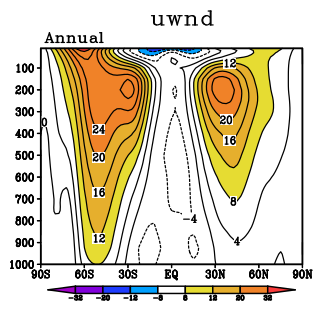
\includegraphics[width=0.5\textwidth]{images/ch03/p17_img01.png}
  \caption{Sea-level pressure (hPa) for (a)~DJF and (b)~JJA. \hisu{DJF: 깊은 Aleutian/Icelandic Low, 강한 시베리아 고기압 ($\sim$1040\,hPa); JJA: 대륙 열적 저기압 (아시아, 북미), 강한 해양 아열대 고기압}}
  \label{fig:ch03-slp-seasonal}
\end{figure}

\begin{remark}[계절별 SLP 대비]
\begin{multicols}{2}
\textgr{DJF (boreal winter):}
\begin{itemize}
  \item 깊은 Aleutian Low
  \item 깊은 Icelandic Low
  \item 강한 Siberian High ($\sim$1040\,hPa)
  \item 강한 pressure gradient $\Rightarrow$ 강한 midlatitude westerlies
\end{itemize}

\columnbreak

\textgr{JJA (boreal summer):}
\begin{itemize}
  \item 대륙 thermal low (Asian, N.\ American)
  \item 강한 해양 subtropical high
  \item 약화된 Aleutian/Icelandic Low
  \item Monsoon circulation이 South/East Asia를 지배
\end{itemize}
\end{multicols}
\end{remark}

\hisu{시베리아 고기압은 DJF에만 존재하는 열적 고기압이다.
여름에는 대륙이 가열되어 열적 저기압으로 바뀐다.}

\begin{hisublock}
\textbf{참고 문헌 가이드:}
\begin{itemize}
  \item Peixoto and Oort (1992), \textit{Physics of Climate}, Ch.7.1 (pp.131--136, 본 PDF에는 목차만 수록) -- SLP의 계절 변동 관측
  \item Hartmann (1994), \textit{Global Physical Climatology}, Ch.6.5 (pp.155--169, 본 PDF에는 목차만 수록) -- 몬순과 대규모 기압 패턴의 계절성
\end{itemize}
\end{hisublock}


% ---------------------------------------------------------------------------------------
\subsection{Wind Seasonal Cycle}
% ---------------------------------------------------------------------------------------

\subsubsection{850\,hPa --- Monsoon Circulation}

\begin{figure}[ht]
  \centering
  % TODO: Extract figure from Ch03 lecture note, page 19--20
  % Description: 850 hPa wind for DJF and JJA.  JJA shows the dramatic
  %   South Asian monsoon: cross-equatorial Somali jet along the East African
  %   coast, westerly inflow into the Indian subcontinent.
  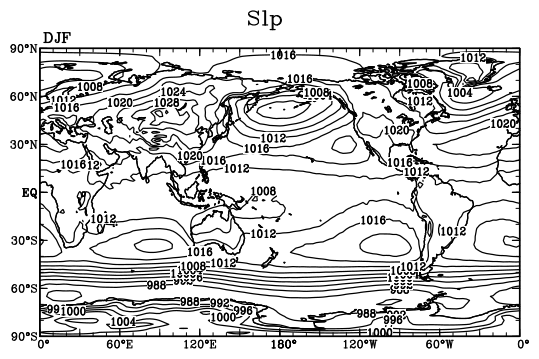
\includegraphics[width=0.6\textwidth]{images/ch03/p19_img01.png}
  \caption{850\,hPa wind (m\,s$^{-1}$) for (a)~DJF and (b)~JJA. \hisu{JJA: 남아시아 몬순의 핵심 --- 적도 횡단 소말리 제트가 동아프리카 해안을 따라 인도 아대륙으로 수분 유입}}
  \label{fig:ch03-wind850-seasonal}
\end{figure}

\begin{remark}[Somali Jet과 monsoon onset]
JJA에, 강력한 \textgr{cross-equatorial low-level jet} --- Somali jet ---이
southern Indian Ocean에서 Indian subcontinent으로 수분을 유입시킨다.
이 jet은 지구상에서 가장 강한 low-level wind feature 중 하나로,
Somalia 해안 부근에서 15--20\,m\,s$^{-1}$에 달한다.
South Asian monsoon onset의 핵심 요소이다.
\end{remark}


\subsubsection{200\,hPa --- Subtropical Jet Intensification}

\begin{figure}[ht]
  \centering
  % TODO: Extract figure from Ch03 lecture note, page 21
  % Description: 200 hPa wind for DJF: strongest NH subtropical jet,
  %   >50 m/s over East Asia.  JJA: jet weakens in NH, SH jet intensifies.
  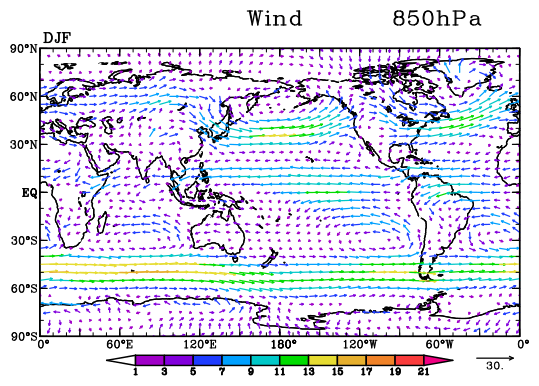
\includegraphics[width=0.6\textwidth]{images/ch03/p21_img01.png}
  \caption{200\,hPa wind (m\,s$^{-1}$) for (a)~DJF and (b)~JJA. \hisu{DJF: NH 아열대 제트 최강, 동아시아 상공 $>$50\,m\,s$^{-1}$; JJA: NH 제트 약화, SH 제트 강화}}
  \label{fig:ch03-wind200-seasonal}
\end{figure}

\hisu{DJF 동아시아 200\,hPa 제트가 50\,m/s를 초과하는 이유:
겨울에는 적도--극 온도 경도가 최대이고, 티벳 고원의 기계적/열적 강제가 합쳐지기 때문이다.}

\begin{hisublock}
\textbf{참고 문헌 가이드:}
\begin{itemize}
  \item Hartmann (1994), \textit{Global Physical Climatology}, Ch.6.5 (pp.155--169, 본 PDF에는 목차만 수록) -- monsoon circulation과 seasonal wind pattern
  \item Peixoto and Oort (1992), \textit{Physics of Climate}, Ch.7.4 (pp.149--161, 본 PDF에는 목차만 수록) -- wind field의 계절 변동 관측
  \item Webster (1987), ``The elementary monsoon'' -- Somali jet과 Asian monsoon의 역학
\end{itemize}
\end{hisublock}


% ---------------------------------------------------------------------------------------
\subsection{Zonal-Mean Zonal Wind --- Seasonal}
% ---------------------------------------------------------------------------------------

\begin{figure}[ht]
  \centering
  % TODO: Extract figure from Ch03 lecture note, page 22
  % Description: Latitude--pressure cross-sections of [u] for DJF and JJA.
  %   DJF: NH jet dramatically intensifies to ~28 m/s, shifted equatorward.
  %   JJA: SH jet intensifies; NH jet weakens and shifts poleward.
  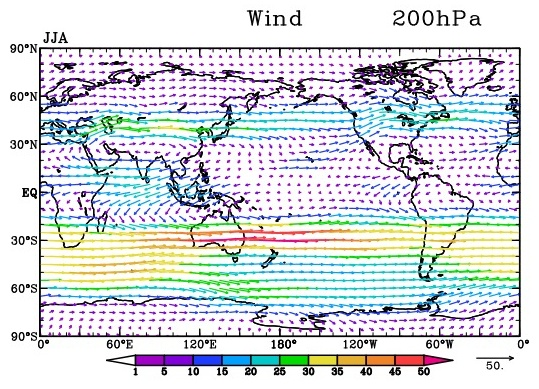
\includegraphics[width=0.6\textwidth]{images/ch03/p22_img01.jpeg}
  \caption{Zonal-mean zonal wind $[\bar{u}]$ (m\,s$^{-1}$) for (a)~DJF and (b)~JJA. \hisu{DJF: NH 제트 강화 ($\sim$28\,m\,s$^{-1}$, 적도 쪽 이동); JJA: SH 제트 강화, NH 제트 약화 및 극 쪽 이동 --- 겨울 반구 온도 경도가 최대}}
  \label{fig:ch03-zmzw-seasonal}
\end{figure}

\begin{remark}[계절별 jet 비대칭]
DJF에 NH subtropical jet은 zonal mean에서 $\sim$28\,m\,s$^{-1}$까지 (국지적으로는 훨씬 더)
극적으로 강화되는 반면, SH jet은 약화된다. JJA에는 이 패턴이 역전된다.
이는 thermal wind relation~\eqref{eq:thermal-wind-ch03}의 직접적 결과이다:
\textgr{winter hemisphere}가 항상 가장 급한 meridional temperature gradient를 가지므로
가장 강한 jet을 형성한다.
\end{remark}


% ---------------------------------------------------------------------------------------
\subsection{Zonal-Mean Meridional Wind --- Seasonal}
% ---------------------------------------------------------------------------------------

\begin{figure}[ht]
  \centering
  % TODO: Extract figure from Ch03 lecture note, page 23
  % Description: [v] cross-section for DJF and JJA.  Clear seasonal
  %   migration of the cross-equatorial Hadley cell: in DJF the dominant
  %   cell has ascent south of the equator, upper-level northward flow,
  %   and descent near 30N.
  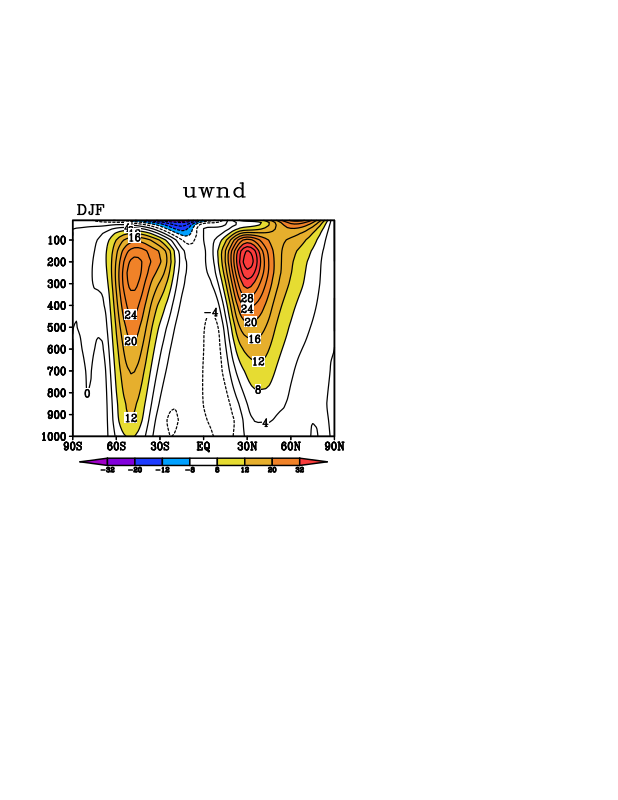
\includegraphics[width=0.6\textwidth]{images/ch03/p23_img01.png}
  \caption{Zonal-mean meridional wind $[\bar{v}]$ (m\,s$^{-1}$) for (a)~DJF and (b)~JJA,
           showing the cross-equatorial Hadley cell. \hisu{해들리 셀의 계절 이동: DJF에는 적도 남쪽 상승, 상층 북향 흐름, $\sim$$30^{\circ}$N 하강; JJA에는 반대}}
  \label{fig:ch03-zmvw-seasonal}
\end{figure}

\begin{hisublock}
계절에 따라 해들리 셀의 상승 지역이 여름 반구 쪽으로 이동한다.
DJF에는 SH에서 상승하고 NH에서 하강하는 ``겨울 셀''이 우세하고,
JJA에는 반대이다.  이 비대칭이 몬순과 ITCZ의 계절 이동을 구동한다.
\end{hisublock}

\begin{remark}[JJA cross-equatorial flow가 DJF보다 강한 이유]
Cross-equatorial Hadley overturning이 JJA에 DJF보다 강한 이유는 다음과 같다:
\begin{enumerate}
\item Asian summer monsoon이 NH subtropics에 강력한 추가 heat source를 제공하여 cross-equatorial pressure gradient를 강화한다.
\item Thermal equator가 JJA에 더 북쪽으로 이동 (Asia 상공 $\sim$20$^\circ$N)하여 DJF ($\sim$10$^\circ$S)보다 더 비대칭적인 forcing을 만든다.
\item Land--sea 분포: NH가 더 많은 land mass를 가지고 있어 계절적 heating contrast가 증폭된다.
\end{enumerate}
\end{remark}
\begin{hisublock}
JJA에 적도 횡단 해들리 순환이 DJF보다 강한 이유:
아시아 여름 몬순이 강력한 추가 열원을 제공하고, 열적 적도가 NH에서 더 멀리 이동하며 ($\sim$20$^\circ$N vs $\sim$10$^\circ$S), NH의 대륙 면적이 더 넓어 계절 가열 대비가 증폭된다.
\end{hisublock}

\begin{hisublock}
\textbf{참고 문헌 가이드:}
\begin{itemize}
  \item Peixoto and Oort (1992), \textit{Physics of Climate}, Ch.7.4 (pp.149--161, 본 PDF에는 목차만 수록) -- zonal-mean wind의 계절 변동 관측
  \item Hartmann (1994), \textit{Global Physical Climatology}, Ch.6.3 (pp.138--149, 본 PDF에는 목차만 수록) -- meridional transport와 Hadley cell의 계절 비대칭
  \item Dima and Wallace (2003), ``On the seasonality of the Hadley cell'' -- cross-equatorial Hadley cell의 계절 비대칭 분석
\end{itemize}
\end{hisublock}


% ---------------------------------------------------------------------------------------
\subsection{Zonal-Mean Temperature}
% ---------------------------------------------------------------------------------------

\begin{figure}[ht]
  \centering
  % TODO: Extract figure from Ch03 lecture note, page 24--25
  % Description: Latitude--pressure cross-sections of [T] for DJF and JJA.
  %   Steepest meridional temperature gradient always in the winter hemisphere.
  %   Tropical tropopause is higher (~100 hPa) and colder (~190 K);
  %   extratropical tropopause is lower (~300 hPa) and warmer (~220 K).
  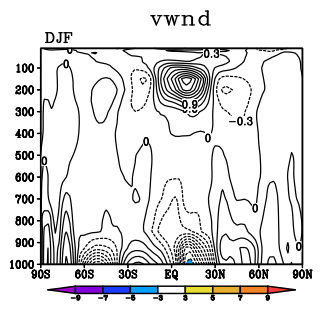
\includegraphics[width=0.6\textwidth]{images/ch03/p24_img01.png}
  \caption{Zonal-mean temperature $[\bar{T}]$ (K) for (a)~DJF and (b)~JJA. \hisu{가장 급한 남북 $T$ 경도는 항상 겨울 반구; 열대 대류권계면: $\sim$100\,hPa, $\sim$190\,K (높고 차가움); 중위도 대류권계면: $\sim$300\,hPa, $\sim$220\,K (낮고 따뜻함)}}
  \label{fig:ch03-zmt-seasonal}
\end{figure}

\begin{definition}[Tropopause structure]
The tropopause --- the boundary between the troposphere and stratosphere --- has a
fundamentally different character in the tropics and extratropics:
\begin{multicols}{2}
\textgr{Tropical tropopause:}
\begin{itemize}
  \item Height: $\sim$100\,hPa ($\sim$16--17\,km)
  \item Temperature: $\sim$190\,K ($-83^{\circ}$C)
  \item Set by deep convective overshooting and radiative balance
\end{itemize}

\columnbreak

\textgr{Extratropical tropopause:}
\begin{itemize}
  \item Height: $\sim$300\,hPa ($\sim$9--12\,km)
  \item Temperature: $\sim$220\,K ($-53^{\circ}$C)
  \item Set by baroclinic eddy mixing and radiative processes
\end{itemize}
\end{multicols}
The global-mean tropospheric lapse rate is approximately
$\Gamma \approx 6.5$\,K\,km$^{-1}$.
\end{definition}


% ---------------------------------------------------------------------------------------
\subsection{Vertical Temperature Profiles}
% ---------------------------------------------------------------------------------------

\begin{figure}[ht]
  \centering
  % TODO: Extract figure from Ch03 lecture note, page 26
  % Description: Vertical profiles of temperature at representative latitudes
  %   (equator, 45N, 75N).  Shows tropical tropopause higher and colder than
  %   extratropical tropopause.  Lapse rate ~6.5 K/km in the troposphere.
  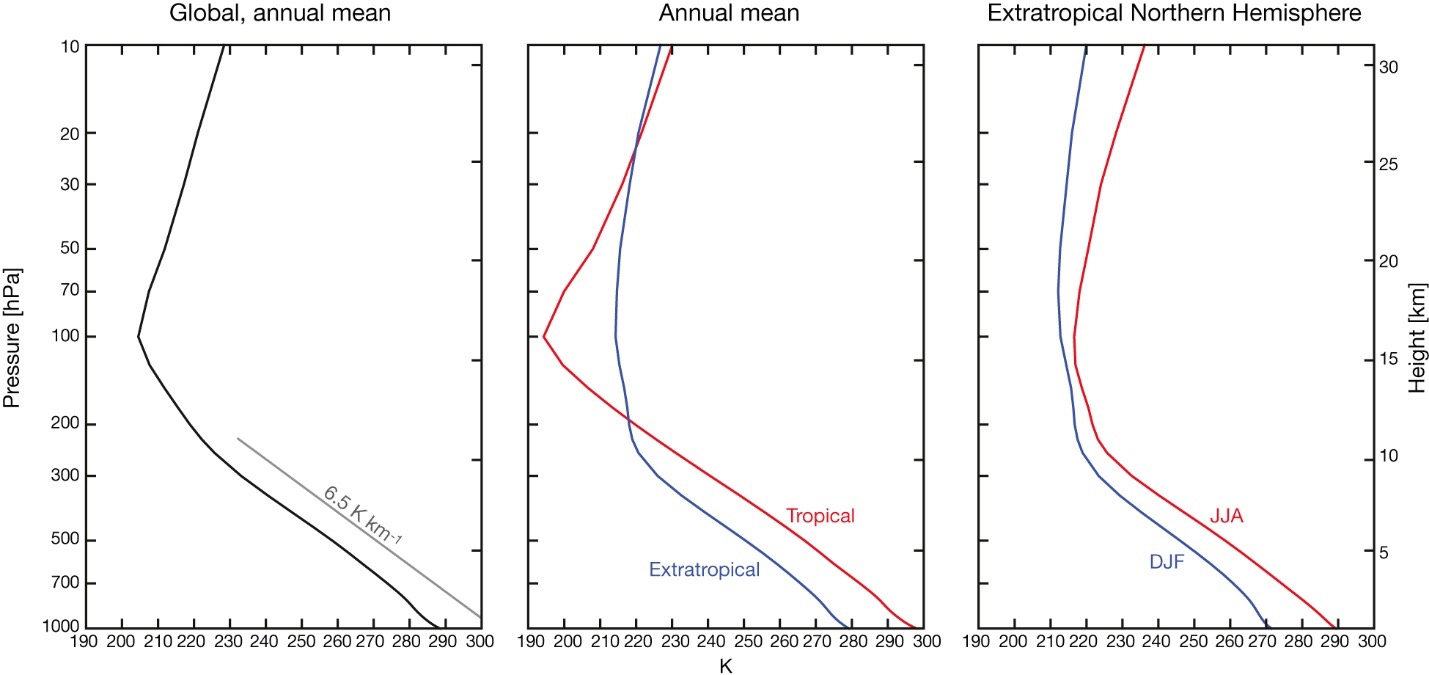
\includegraphics[width=\textwidth]{images/ch03/p26_img01.jpeg}
  \caption{Vertical temperature profiles at representative latitudes (적도, $45^{\circ}$N, $75^{\circ}$N). \hisu{열대 대류권계면이 중위도보다 높고 차가움; 대류권 감률 $\sim$6.5\,K\,km$^{-1}$}}
  \label{fig:ch03-temp-profiles}
\end{figure}

\hisu{열대 대류권계면이 더 높고 더 차가운 것은, 깊은 대류(deep convection)가
공기를 높이까지 밀어올리기 때문이다.  반면 중위도 대류권계면은 경압 불안정에 의한
에디 혼합이 결정한다.}

\begin{hisublock}
\textbf{참고 문헌 가이드:}
\begin{itemize}
  \item Peixoto and Oort (1992), \textit{Physics of Climate}, Ch.7.2 (pp.137--143, 본 PDF에는 목차만 수록) -- temperature의 관측 분포 및 대류권계면 구조
  \item Hartmann (1994), \textit{Global Physical Climatology}, Ch.6.3 (pp.138--149, 본 PDF에는 목차만 수록) -- meridional temperature gradient와 계절 변동
  \item Marshall and Plumb (2008), \textit{Atmosphere, Ocean and Climate Dynamics}, Ch.5.1 (pp.62--67, PDF pp.83--88) -- 대기의 radiative forcing과 온도 구조
\end{itemize}
\end{hisublock}


% ---------------------------------------------------------------------------------------
\subsection{Quasi-Biennial Oscillation (QBO)}
\label{sec:ch03-qbo}
% ---------------------------------------------------------------------------------------

\begin{figure}[ht]
  \centering
  % TODO: Extract figure from Ch03 lecture note, page 27--28
  % Description: Time--height diagram of equatorial stratospheric temperature
  %   (or zonal wind) anomalies, showing the QBO.  Alternating easterly and
  %   westerly regimes descend from ~10 hPa to ~70 hPa with a period of
  %   ~26 months.  Amplitude ~3 K in temperature.
  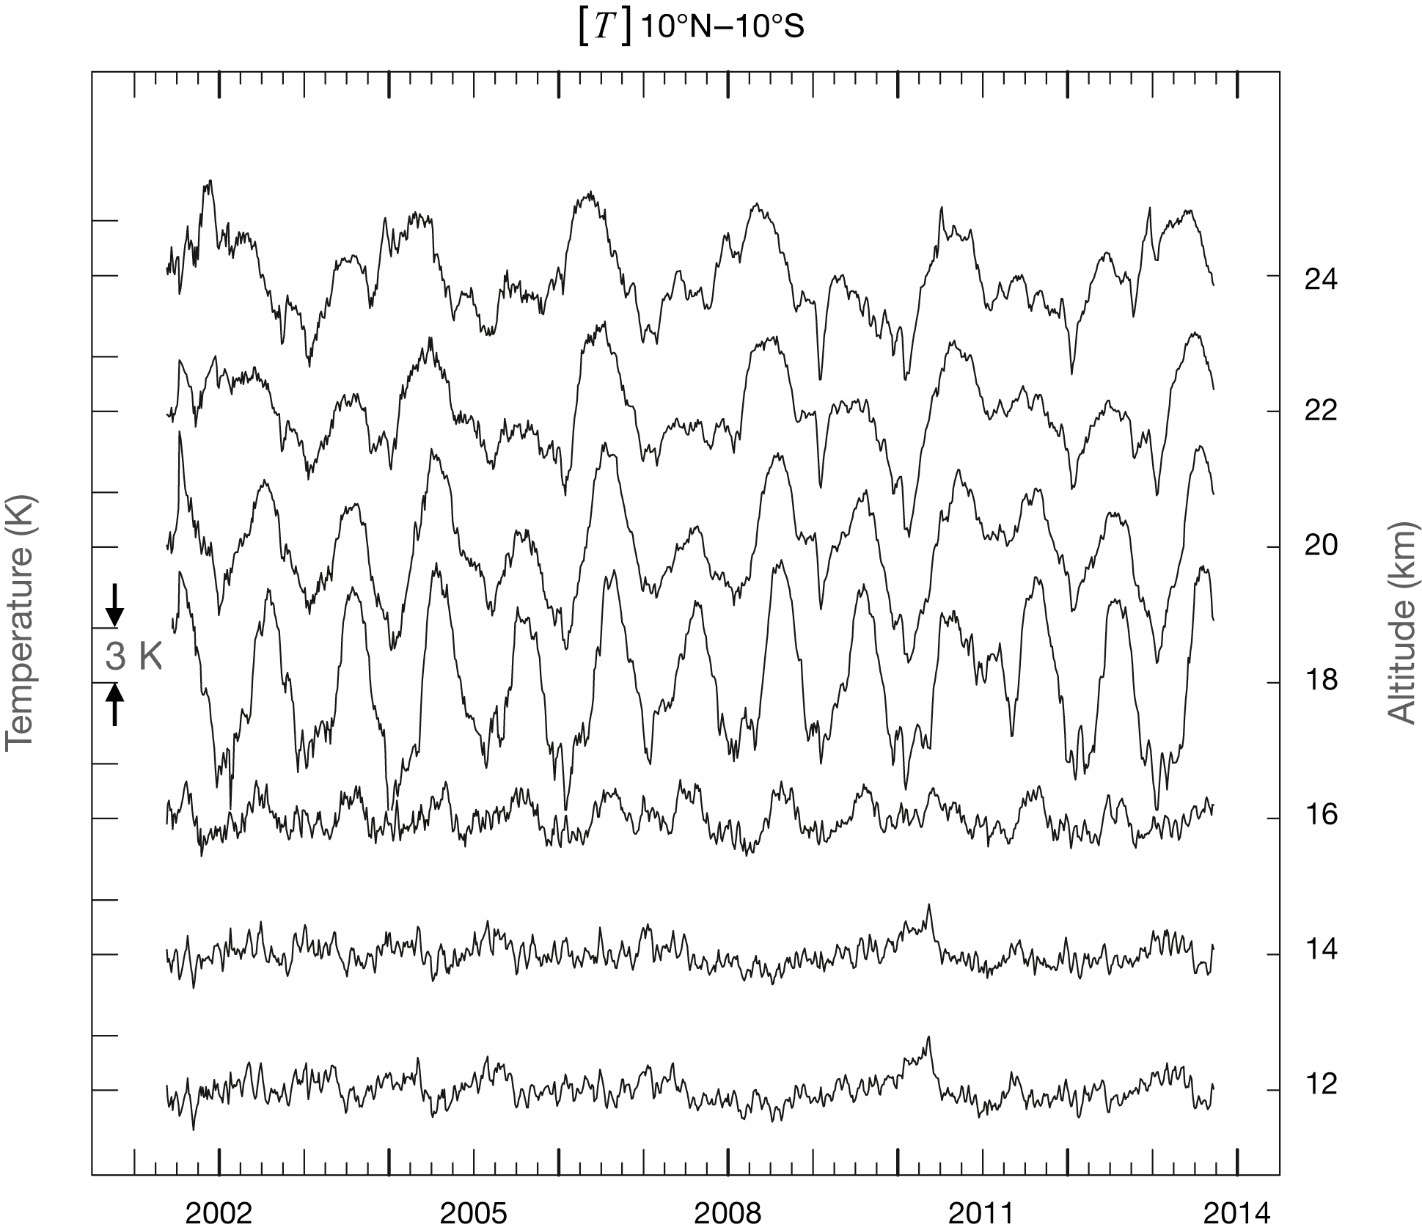
\includegraphics[width=0.7\textwidth]{images/ch03/p27_img01.jpeg}
  \caption{Quasi-biennial oscillation (QBO) in equatorial stratospheric temperature anomalies (시간--고도 다이어그램). \hisu{동풍/서풍 레짐이 $\sim$10\,hPa에서 $\sim$70\,hPa로 하강, 주기 $\sim$26개월, 진폭 $\sim$3\,K}}
  \label{fig:ch03-qbo}
\end{figure}

\begin{definition}[Quasi-Biennial Oscillation (QBO)]
The QBO is a quasi-periodic oscillation of the equatorial stratospheric zonal wind between
easterly and westerly regimes, with:
\begin{itemize}
  \item \textgr{Period}: $\sim$26--28 months (hence ``quasi-biennial'')
  \item \textgr{Amplitude}: $\sim$20--30\,m\,s$^{-1}$ in zonal wind; $\sim$3\,K in temperature
  \item \textgr{Vertical propagation}: phases descend from $\sim$10\,hPa to $\sim$70\,hPa
  \item \textgr{Mechanism}: driven by the interaction of vertically propagating equatorial
        waves (Kelvin and mixed Rossby--gravity waves) with the mean flow
\end{itemize}
\end{definition}

\begin{hisublock}
QBO = 준 2년 진동.  적도 성층권에서 동풍과 서풍이 약 2년 주기로 교대한다.
이것은 대류권에서 발생한 적도 파동(Kelvin wave, MRG wave)이 성층권으로
전파되어 평균류를 가속/감속시키는 wave--mean flow interaction의 결과이다.
QBO는 몬순, 극소용돌이 등 대류권 기후에도 원격 영향을 미친다.
\end{hisublock}

\begin{hisublock}
\textbf{참고 문헌 가이드:}
\begin{itemize}
  \item Baldwin et al.\ (2001), ``The quasi-biennial oscillation'', \textit{Rev.\ Geophys.} -- QBO의 종합적 리뷰
  \item Holton and Lindzen (1972), ``An updated theory for the quasi-biennial cycle'' -- wave--mean flow interaction에 의한 QBO 메커니즘의 기초 이론
  \item Peixoto and Oort (1992), \textit{Physics of Climate}, Ch.7.4 (pp.149--161, 본 PDF에는 목차만 수록) -- 성층권 순환 관측
\end{itemize}
\end{hisublock}


% ---------------------------------------------------------------------------------------
\subsection{ITCZ Seasonal Migration}
% ---------------------------------------------------------------------------------------

\begin{figure}[ht]
  \centering
  % TODO: Extract figure from Ch03 lecture note, page 29
  % Description: Latitude--month cross-section of zonal-mean omega at 500 hPa,
  %   showing the seasonal migration of the ITCZ (band of negative omega).
  %   Ascent migrates from ~5S in DJF to ~10N in JJA over the continents.
  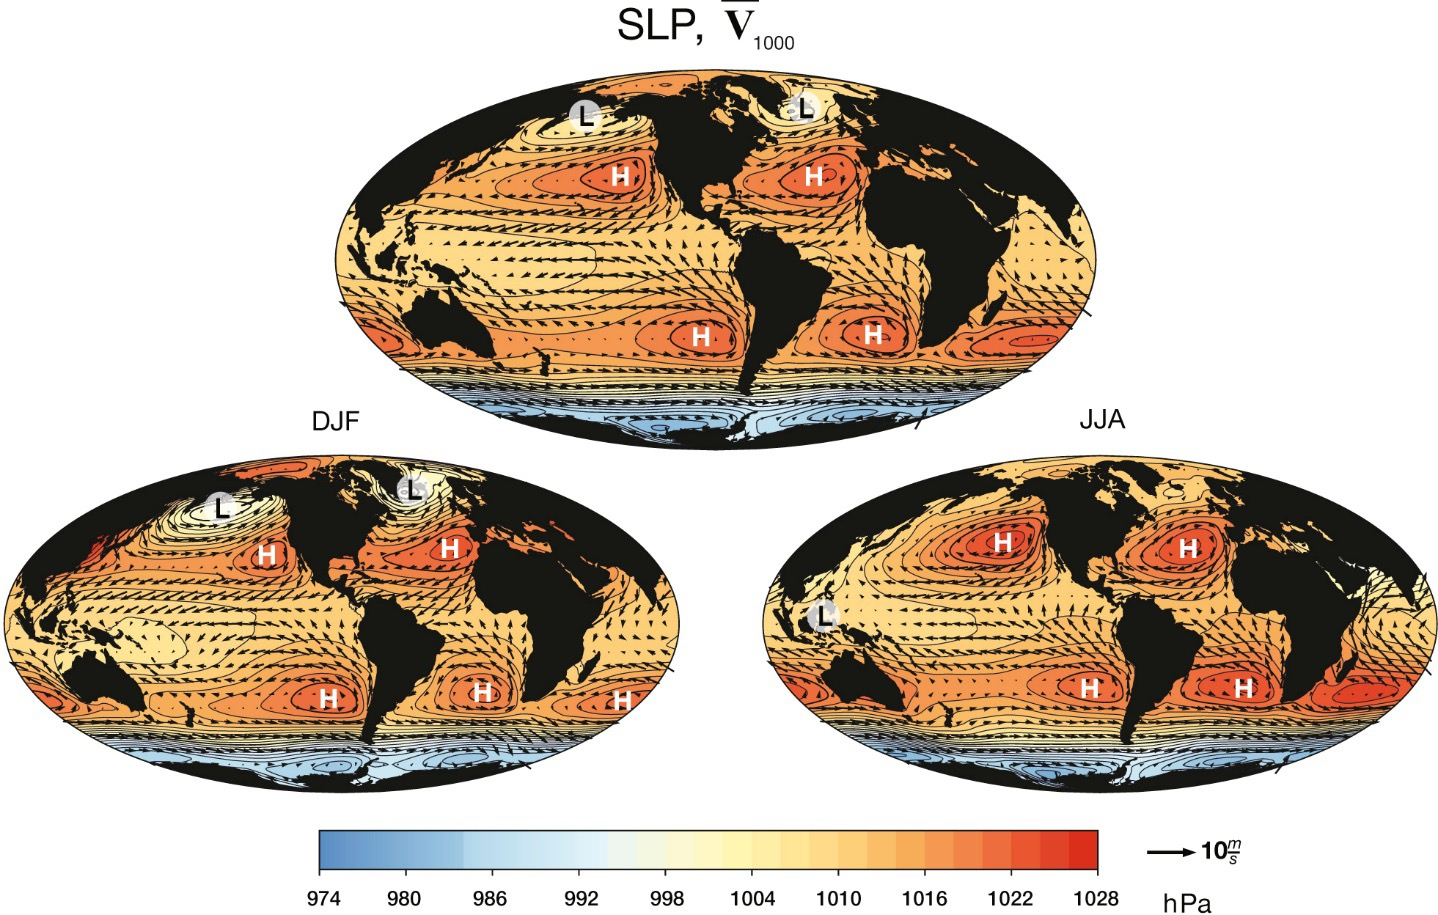
\includegraphics[width=0.85\textwidth]{images/ch03/p29_img01.jpeg}
  \caption{Latitude--month cross-section of $[\bar{\omega}]$ at 500\,hPa, illustrating
           the seasonal migration of the ITCZ. \hisu{상승 운동($\omega<0$) 대역이 DJF $\sim$$5^{\circ}$S에서 JJA $\sim$$10^{\circ}$N으로 이동 (대륙 위에서 더 큰 폭)}}
  \label{fig:ch03-itcz-migration}
\end{figure}

\begin{remark}[ITCZ 이동]
ITCZ (Intertropical Convergence Zone)는 maximum insolation의 seasonal cycle을
$\sim$1--2개월의 지연으로 따른다:
\begin{itemize}
  \item DJF: ITCZ가 $\sim$$5^{\circ}$S (대륙 위) $\sim$ $\sim$$5^{\circ}$N (해양 위) 부근에 위치
  \item JJA: ITCZ가 대륙 위에서 $\sim$$10^{\circ}$N까지 이동 (South Asia에서는 $25^{\circ}$N까지
        --- monsoon)
  \item ITCZ는 해양보다 대륙 위에서 적도로부터 더 멀리 이동하는데, 이는 land surface의
        thermal inertia가 더 낮기 때문이다.
\end{itemize}
\end{remark}

\hisu{ITCZ의 계절 이동은 강수와 대규모 순환의 계절 변동을 이해하는 열쇠이다.
ITCZ가 $5^{\circ}$N에서 $25^{\circ}$N까지 이동하는 것이 바로 아시아 몬순의 본질이다.}

\begin{hisublock}
\textbf{참고 문헌 가이드:}
\begin{itemize}
  \item Hartmann (1994), \textit{Global Physical Climatology}, Ch.6.5 (pp.155--169, 본 PDF에는 목차만 수록) -- ITCZ, monsoon, Walker circulation의 관측
  \item Peixoto and Oort (1992), \textit{Physics of Climate}, Ch.7.6 (pp.165--175, 본 PDF에는 목차만 수록) -- precipitation과 evaporation의 전구 분포
  \item Schneider et al.\ (2014), ``Migrations and dynamics of the intertropical convergence zone'', \textit{Nature} -- ITCZ 이동의 에너지 균형 관점
\end{itemize}
\end{hisublock}


% =======================================================================================
\section{Precipitation}
\label{sec:ch03-precip}
% =======================================================================================

\subsection{Annual-Mean Precipitation}

\begin{figure}[ht]
  \centering
  % TODO: Extract figure from Ch03 lecture note, page 30--31
  % Description: Annual-mean precipitation (mm/day) from GPCP or CMAP.
  %   Key features: ITCZ (7--13 mm/day), warm pool / Maritime Continent
  %   (>9 mm/day), SPCZ extending SE from warm pool, midlatitude storm
  %   tracks (3--5 mm/day), arid subtropics.
  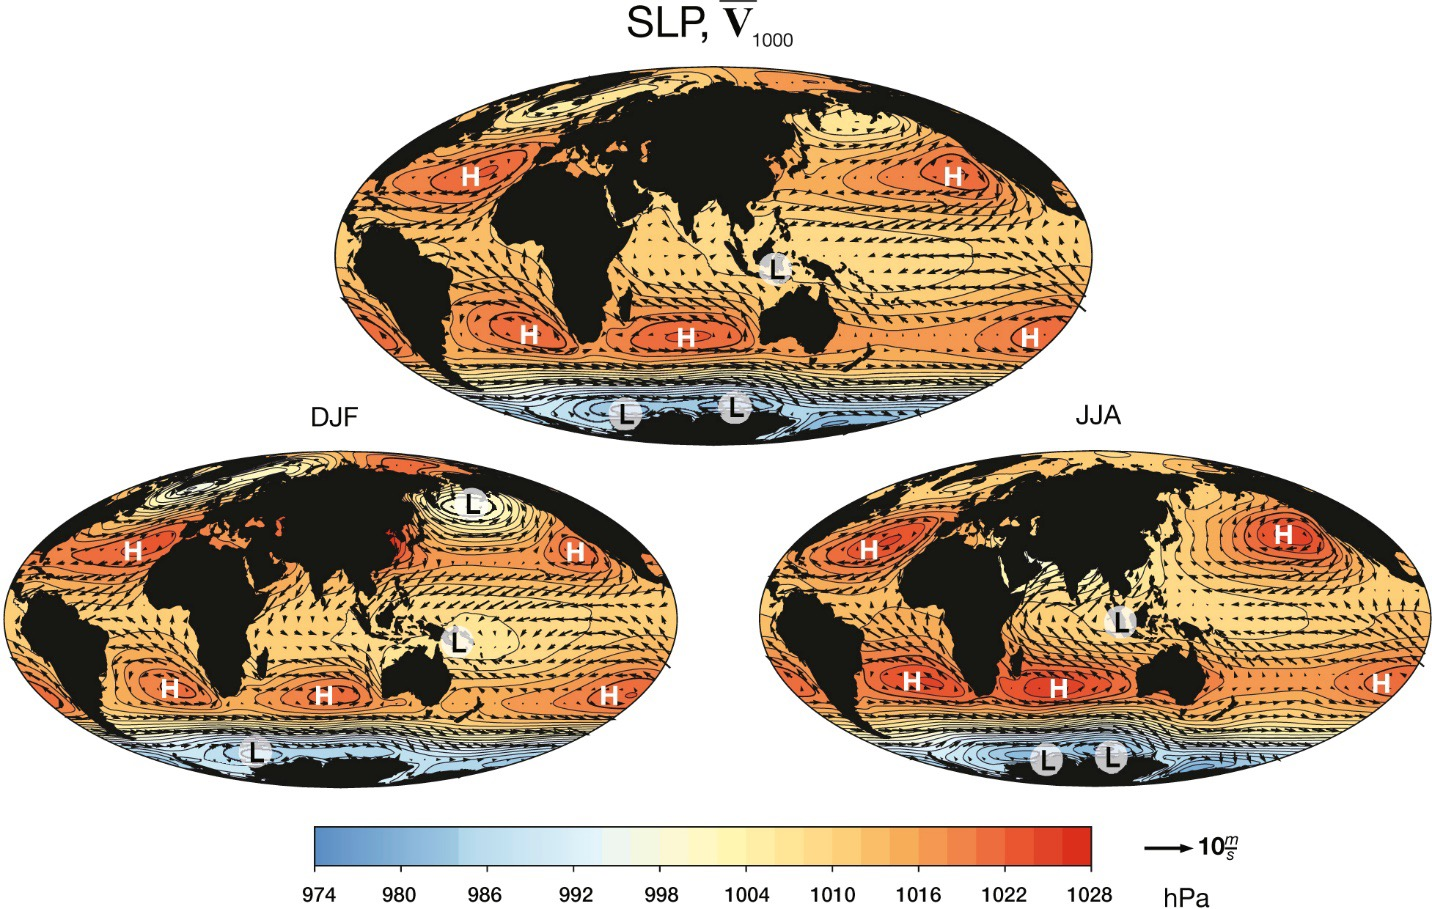
\includegraphics[width=0.85\textwidth]{images/ch03/p30_img01.jpeg}
  \caption{Annual-mean precipitation rate (mm\,day$^{-1}$, GPCP/CMAP). \hisu{ITCZ (7--13\,mm\,day$^{-1}$), warm pool/해양대륙 ($>$9), SPCZ, 중위도 폭풍 경로 (3--5), 아열대 건조대 (해들리 셀 하강)}}
  \label{fig:ch03-precip-ann}
\end{figure}

\begin{definition}[Major Precipitation Features]
\begin{itemize}
  \item \textgr{ITCZ} (Intertropical Convergence Zone): a narrow band near $5$--$10^{\circ}$N with
        precipitation rates of 7--13\,mm\,day$^{-1}$, driven by low-level convergence and deep
        convection.
  \item \textgr{Warm pool / Maritime Continent}: the region of highest annual-mean precipitation
        ($>$9\,mm\,day$^{-1}$), centred over the western Pacific and Indonesia.
  \item \textgr{SPCZ} (South Pacific Convergence Zone): extends south-eastward from the warm pool
        into the subtropical South Pacific.
  \item \textgr{Midlatitude storm tracks}: moderate precipitation (3--5\,mm\,day$^{-1}$) associated
        with transient baroclinic eddies, especially over the North Pacific and North Atlantic.
  \item \textgr{Arid subtropics}: the descending branches of the Hadley cell suppress precipitation
        in the subtropical belt ($\sim$$15$--$30^{\circ}$\,N/S).
\end{itemize}
\end{definition}


\subsection{Precipitation and Vertical Motion}

\begin{figure}[ht]
  \centering
  % TODO: Extract figure from Ch03 lecture note, page 32
  % Description: Scatter plot or co-located maps of precipitation vs. 500 hPa
  %   omega, showing strong spatial correlation: regions of ascent (omega < 0)
  %   are regions of high precipitation.
  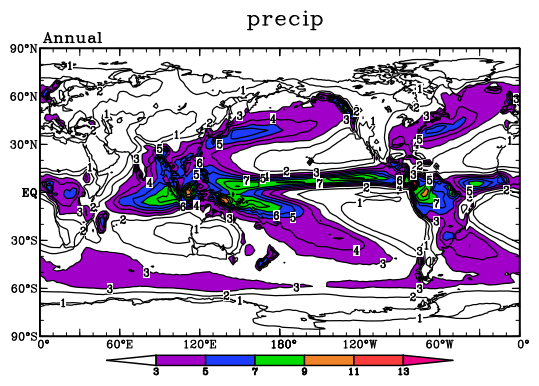
\includegraphics[width=0.85\textwidth]{images/ch03/p32_img01.png}
  \caption{Spatial relationship between precipitation and 500\,hPa $\omega$. \hisu{상승 운동($\omega<0$) 지역 = 다우 지역; 강한 공간 상관 --- 대규모 상승이 단열 냉각, 포화, 응결, 강수를 유발}}
  \label{fig:ch03-precip-omega}
\end{figure}

\begin{remark}[강수--연직 운동 연결]
연평균 precipitation과 mid-tropospheric ascent ($\omega_{500} < 0$) 사이에는 강한 공간 상관이 존재한다.
이는 근본적 메커니즘을 반영한다: large-scale \textgr{upward motion}이
adiabatic cooling, saturation, condensation, 그리고 precipitation을 유발한다.
반대로, large-scale descent 지역은 건조하다.
\end{remark}

\hisu{강수 = 상승 운동과 밀접하게 연결.  특히 ITCZ와 warm pool에서 $\omega < 0$이 강하고
강수가 많다.  아열대 고기압 지역에서는 $\omega > 0$ (하강)이고 강수가 적다.}


\subsection{Seasonal Precipitation}

\begin{figure}[ht]
  \centering
  % TODO: Extract figure from Ch03 lecture note, page 33--34
  % Description: Precipitation for DJF and JJA.  JJA: ITCZ shifts far north,
  %   intense rainfall over South/Southeast Asia, West Africa (monsoons).
  %   DJF: ITCZ shifts south, maritime continent rainfall broadens, South
  %   American and Australian monsoons active.
  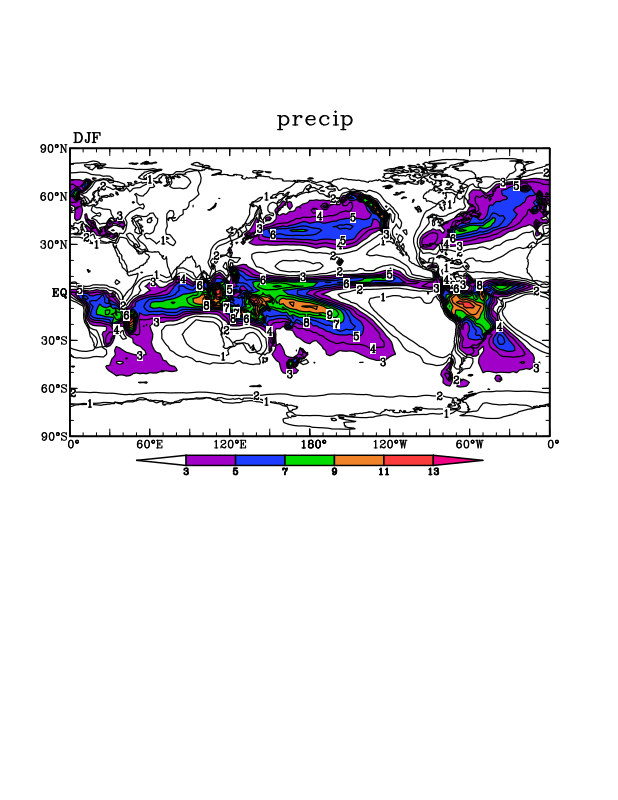
\includegraphics[width=0.85\textwidth]{images/ch03/p33_img01.png}
  \caption{Precipitation rate (mm\,day$^{-1}$) for (a)~DJF and (b)~JJA. \hisu{JJA: ITCZ 북상, 남/동남아시아-서아프리카 몬순 강우; DJF: ITCZ 남하, 해양대륙 강수 확대, 남미/호주 몬순 활성화}}
  \label{fig:ch03-precip-seasonal}
\end{figure}

\begin{remark}[계절별 강수 패턴]
\begin{multicols}{2}
\textgr{JJA:}
\begin{itemize}
  \item ITCZ가 크게 북상
  \item Asian monsoon: India, Bangladesh, Southeast Asia에 강한 강우
  \item West African monsoon 활성화
  \item NH storm track 약화
\end{itemize}

\columnbreak

\textgr{DJF:}
\begin{itemize}
  \item ITCZ가 적도 부근 또는 남쪽
  \item Maritime Continent 강수 확대
  \item Australian 및 South American monsoon
  \item NH storm track 강화 $\Rightarrow$ midlatitude precipitation 증가
\end{itemize}
\end{multicols}
\end{remark}


\subsection{Diabatic Heating Rate}

\begin{figure}[ht]
  \centering
  % TODO: Extract figure from Ch03 lecture note, page 35
  % Description: Map of column-integrated diabatic heating rate Q (850--500 hPa).
  %   Positive values in ITCZ and warm pool (latent heat release dominates
  %   radiative cooling); negative values in subtropics (radiative cooling
  %   dominates).
  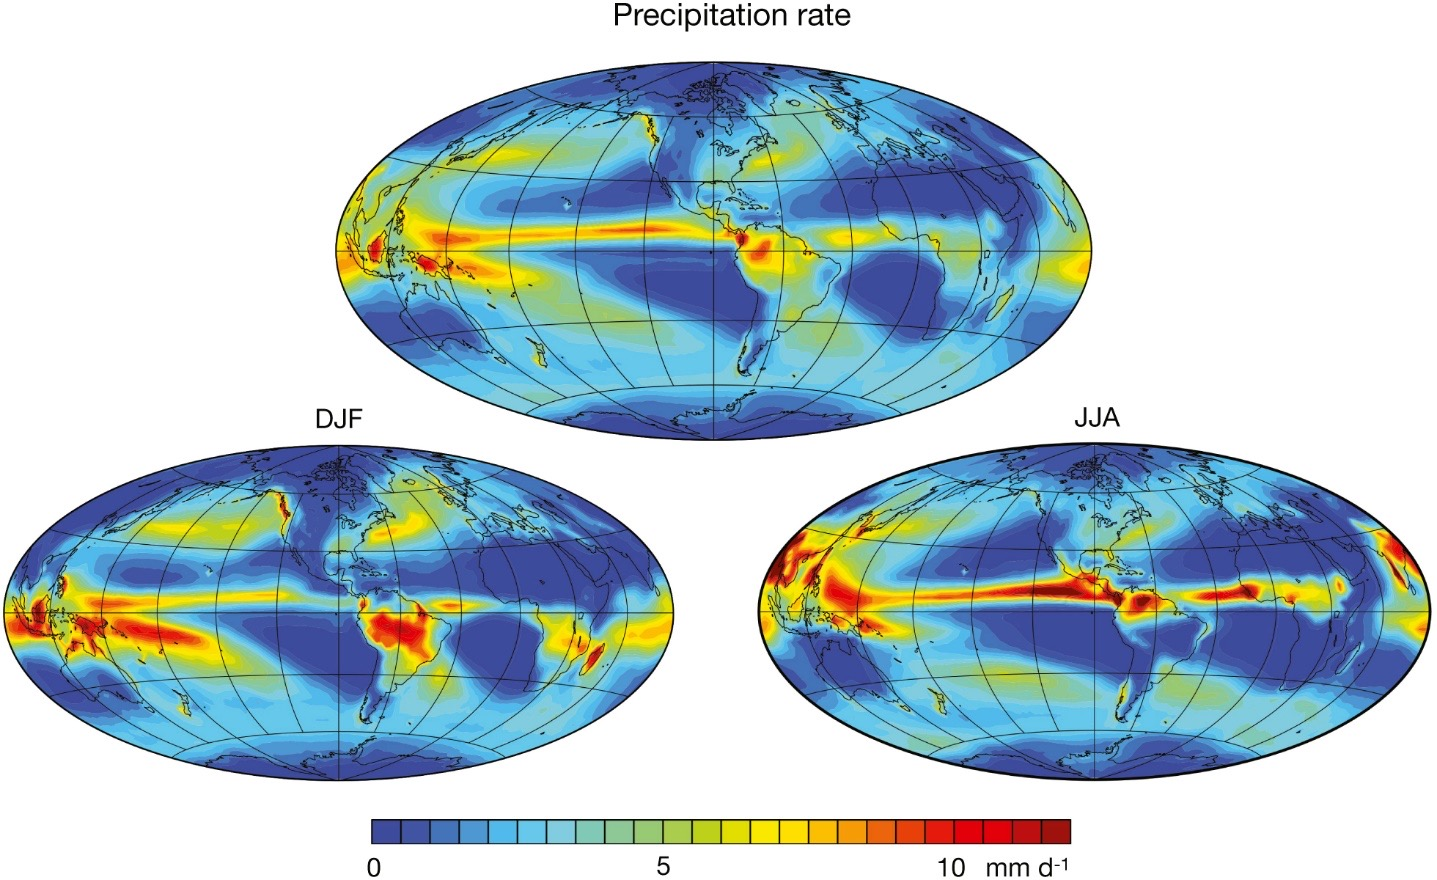
\includegraphics[width=0.85\textwidth]{images/ch03/p35_img01.jpeg}
  \caption{Diabatic heating rate $Q$ averaged over the 850--500\,hPa layer (K\,day$^{-1}$). \hisu{$Q>0$: ITCZ/warm pool (잠열 방출이 복사 냉각 초과); $Q<0$: 아열대 (맑은 하늘 복사 냉각이 우세)}}
  \label{fig:ch03-diabatic}
\end{figure}

\begin{remark}[Diabatic heating: latent heat vs.\ radiative cooling]
하층--중층 대류권에서 net diabatic heating rate는
\textgr{latent heat release} (양, precipitation과 연관)와
\textgr{radiative cooling} (음, 특히 우주로의 longwave emission) 사이의 잔차이다.
ITCZ와 warm pool에서는 latent heating이 강하게 우세하여 ($Q > 0$),
맑은 하늘의 subtropics에서는 radiative cooling이 우세하다 ($Q < 0$).
\end{remark}

\begin{hisublock}
\textbf{참고 문헌 가이드:}
\begin{itemize}
  \item Peixoto and Oort (1992), \textit{Physics of Climate}, Ch.7.6 (pp.165--175, 본 PDF에는 목차만 수록) -- precipitation, evaporation의 전구 분포와 diabatic heating
  \item Hartmann (1994), \textit{Global Physical Climatology}, Ch.6.3, 6.5 (pp.138--169, 본 PDF에는 목차만 수록) -- 강수 패턴과 대규모 순환의 연결
  \item Xie and Arkin (1997), ``Global precipitation: A 17-year monthly analysis'' -- CMAP 강수 기후학
\end{itemize}
\end{hisublock}


% =======================================================================================
\section{Sea Surface Temperature (SST)}
\label{sec:ch03-sst}
% =======================================================================================

\subsection{Annual-Mean SST Distribution}

\begin{figure}[ht]
  \centering
  % TODO: Extract figure from Ch03 lecture note, page 36--37
  % Description: Annual-mean SST (deg C).  Warm pool in western Pacific (>28C),
  %   cold tongue in eastern equatorial Pacific (~22--24C), western boundary
  %   currents creating sharp SST gradients (Gulf Stream, Kuroshio), eastern
  %   boundary upwelling zones (cold SST off California, Peru, West Africa).
  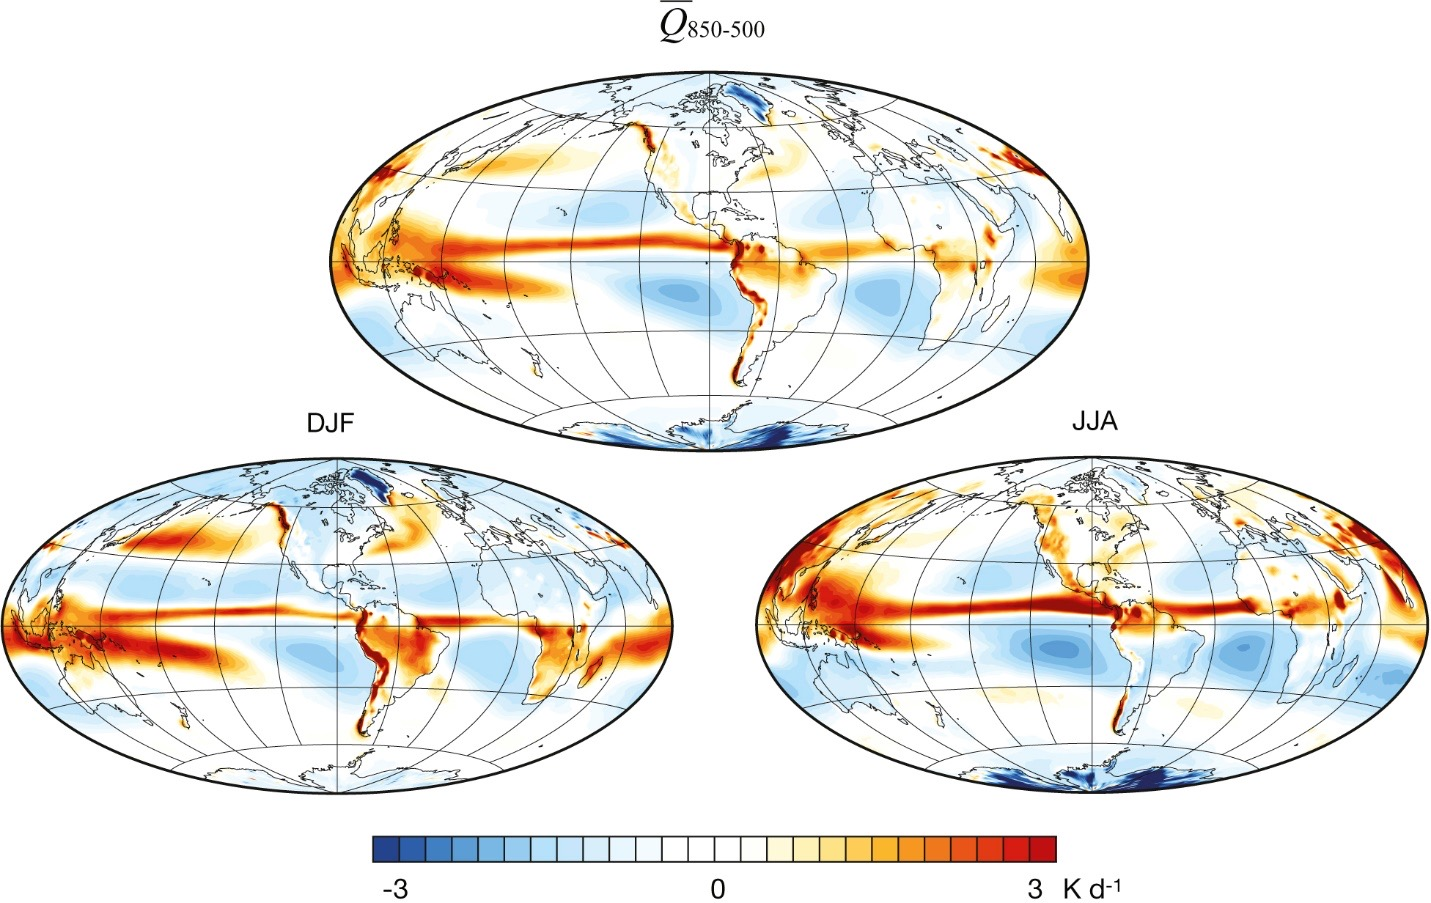
\includegraphics[width=0.85\textwidth]{images/ch03/p36_img01.jpeg}
  \caption{Annual-mean sea surface temperature ($^{\circ}$C). \hisu{서태평양 warm pool ($>$$28^{\circ}$C), 동적도태평양 cold tongue ($\sim$22--24$^{\circ}$C, 적도 용승), 서안 경계류 (Gulf Stream, Kuroshio)의 급경사 SST 전선, 동안 용승대 (차가운 SST)}}
  \label{fig:ch03-sst-ann}
\end{figure}

\begin{definition}[Key SST Features]
\begin{itemize}
  \item \textgr{Warm pool} (western Pacific, $>$28$^{\circ}$C): the warmest open-ocean waters on Earth,
        driven by the accumulation of warm water by the trade winds and weak upwelling.
  \item \textgr{Cold tongue} (eastern equatorial Pacific, $\sim$22--24$^{\circ}$C): maintained by
        equatorial upwelling driven by the easterly trade winds (Ekman divergence).
  \item \textgr{Western boundary currents}: the Gulf Stream and Kuroshio create sharp SST fronts
        ($\sim$$5$--$10^{\circ}$C across $\sim$100\,km).
  \item \textgr{Eastern boundary upwelling}: cold SST off the coasts of California, Peru/Chile,
        and Northwest Africa, driven by equatorward winds and offshore Ekman transport.
\end{itemize}
\end{definition}

\hisu{SST 분포의 동서 비대칭: 서태평양 warm pool vs.\ 동태평양 cold tongue.
이 비대칭은 무역풍(trade winds)에 의해 유지되며,
ENSO 현상에서 이 비대칭이 약화/강화되면서 기후 변동이 발생한다.}


% ---------------------------------------------------------------------------------------
\subsection{SST and Precipitation}
% ---------------------------------------------------------------------------------------

\begin{figure}[ht]
  \centering
  % TODO: Extract figure from Ch03 lecture note, page 38--39
  % Description: Overlay or side-by-side comparison of SST and precipitation.
  %   Heavy rainfall over the warmest SSTs (warm pool), but also shows that
  %   high SST alone is insufficient --- need large-scale convergence.
  %   Eastern equatorial Pacific has warm SST but less rainfall than western
  %   Pacific.
  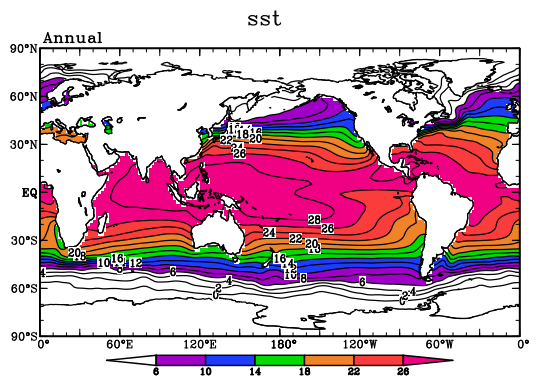
\includegraphics[width=0.6\textwidth]{images/ch03/p38_img01.png}
  \caption{Relationship between SST and precipitation.  Heavy rainfall occurs over the
           warmest SSTs, but convergence is also required. \hisu{고SST만으로는 불충분 --- 대규모 하층 수렴이 필요; 동적도태평양: SST $>$$26^{\circ}$C이지만 Walker 순환 하강으로 강수 적음}}
  \label{fig:ch03-sst-precip}
\end{figure}

\begin{remark}[SST--precipitation 관계]
Precipitation이 가장 따뜻한 SST 위에 집중되지만, \textgr{높은 SST만으로는
충분하지 않다}. 두 가지 조건이 충족되어야 한다:
\begin{enumerate}
  \item SST가 deep convection을 지원하기 위해 $\sim$26--27$^{\circ}$C의 threshold를 초과해야 한다.
  \item \textgr{Large-scale low-level convergence}가 존재하여 moisture flux convergence를 제공하고
        convective instability를 유발해야 한다.
\end{enumerate}
동적도 태평양은 SST $>$ 26$^{\circ}$C인 경우가 많지만, Walker circulation이
low-level divergence를 구동하기 때문에 precipitation은 상대적으로 적다.
\end{remark}

\begin{hisublock}
SST만 높다고 강수가 오는 건 아니다 --- 대규모 수렴도 반드시 필요하다.
서태평양 warm pool에서는 SST가 높고 수렴도 있어서 강수가 강하지만,
동태평양에서는 SST가 비교적 따뜻해도 하강 기류(Walker circulation의 하강 지역)
때문에 강수가 적다.
이것은 열대 기후를 이해하는 데 핵심적인 개념이다.
\end{hisublock}


% ---------------------------------------------------------------------------------------
\subsection{SST and Surface Winds}
% ---------------------------------------------------------------------------------------

\begin{figure}[ht]
  \centering
  % TODO: Extract figure from Ch03 lecture note, page 40--41
  % Description: SST overlaid with surface wind vectors, showing the trade
  %   winds driving equatorial upwelling (cold tongue), Ekman transport, and
  %   the relationship between wind-driven ocean circulation and SST
  %   distribution.
  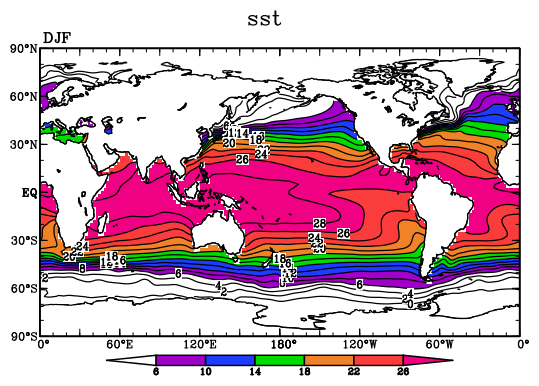
\includegraphics[width=0.6\textwidth]{images/ch03/p40_img01.png}
  \caption{SST ($^{\circ}$C) with surface wind vectors, illustrating the wind--SST coupling. \hisu{무역풍 $\rightarrow$ 적도 Ekman 발산/용승 $\rightarrow$ cold tongue 유지; 따뜻한 SST $\rightarrow$ 경계층 안정도 감소 $\rightarrow$ 지표 바람 강화 (양방향 결합)}}
  \label{fig:ch03-sst-wind}
\end{figure}

\begin{remark}[SST--wind coupling]
SST와 surface wind의 관계는 근본적으로 \textgr{양방향}이다:
\begin{itemize}
  \item \textgr{Wind $\rightarrow$ SST}: trade wind가 equatorial Ekman divergence와
        upwelling을 구동하여 cold tongue를 유지한다. Wind stress curl은 subtropical gyre
        circulation과 western boundary current를 구동한다.
  \item \textgr{SST $\rightarrow$ wind}: 따뜻한 SST는 boundary layer의 atmospheric static stability를 감소시켜
        surface turbulence를 강화하고, free troposphere에서 하향으로 momentum mixing을 촉진하여
        warm SST front 위에서 surface wind를 국지적으로 강화한다.
\end{itemize}
\end{remark}

\begin{hisublock}
무역풍이 적도 용승(equatorial upwelling)을 일으켜 cold tongue를 유지하고,
cold tongue가 다시 동서 기압 경도를 강화하여 무역풍을 유지하는 양의 피드백 루프가 존재한다
(Bjerknes feedback).  이 피드백이 약해지면 El Ni\~{n}o가 발생한다.
\end{hisublock}

\begin{hisublock}
\textbf{참고 문헌 가이드:}
\begin{itemize}
  \item Hartmann (1994), \textit{Global Physical Climatology}, Ch.6.5 (pp.155--169, 본 PDF에는 목차만 수록) -- Walker circulation, ENSO, SST--대기 coupling
  \item Peixoto and Oort (1992), \textit{Physics of Climate}, Ch.7 (pp.131--175, 본 PDF에는 목차만 수록) -- 해양--대기 상호작용의 관측적 기초
  \item Marshall and Plumb (2008), \textit{Atmosphere, Ocean and Climate Dynamics}, Ch.5.3 (pp.70--73, PDF pp.91--94) -- moisture와 SST의 meridional structure
  \item Bjerknes (1969), ``Atmospheric teleconnections from the equatorial Pacific'' -- SST--wind coupling과 ENSO의 고전적 논문
\end{itemize}
\end{hisublock}

% =======================================================================================
\section{Surface (Skin) Temperature Climatology}
\label{sec:ch03-skin-temp}
% =======================================================================================

\textgr{Skin temperature}란 지표면 자체의 온도로, 대기 하층 기온과는 구별된다.
위성 관측에서 직접 측정되며, 대륙 위에서는 land surface temperature (LST),
해양 위에서는 SST에 해당한다.

\subsection{DJF and JJA Skin Temperature Distribution}

\begin{figure}[ht]
  \centering
  % TODO: Use the skin temperature figure from HW3 or extract from lecture notes
  % Description: Global skin temperature maps for DJF and JJA.
  %   DJF: extremely cold Siberia/Canada (-30 to -40C), warm SH continents,
  %        tropics warm, Antarctica very cold.
  %   JJA: Sahara/Arabian peninsula hottest (>40C), northern continents warm,
  %        Southern Ocean cold, tropical oceans remain warm.
  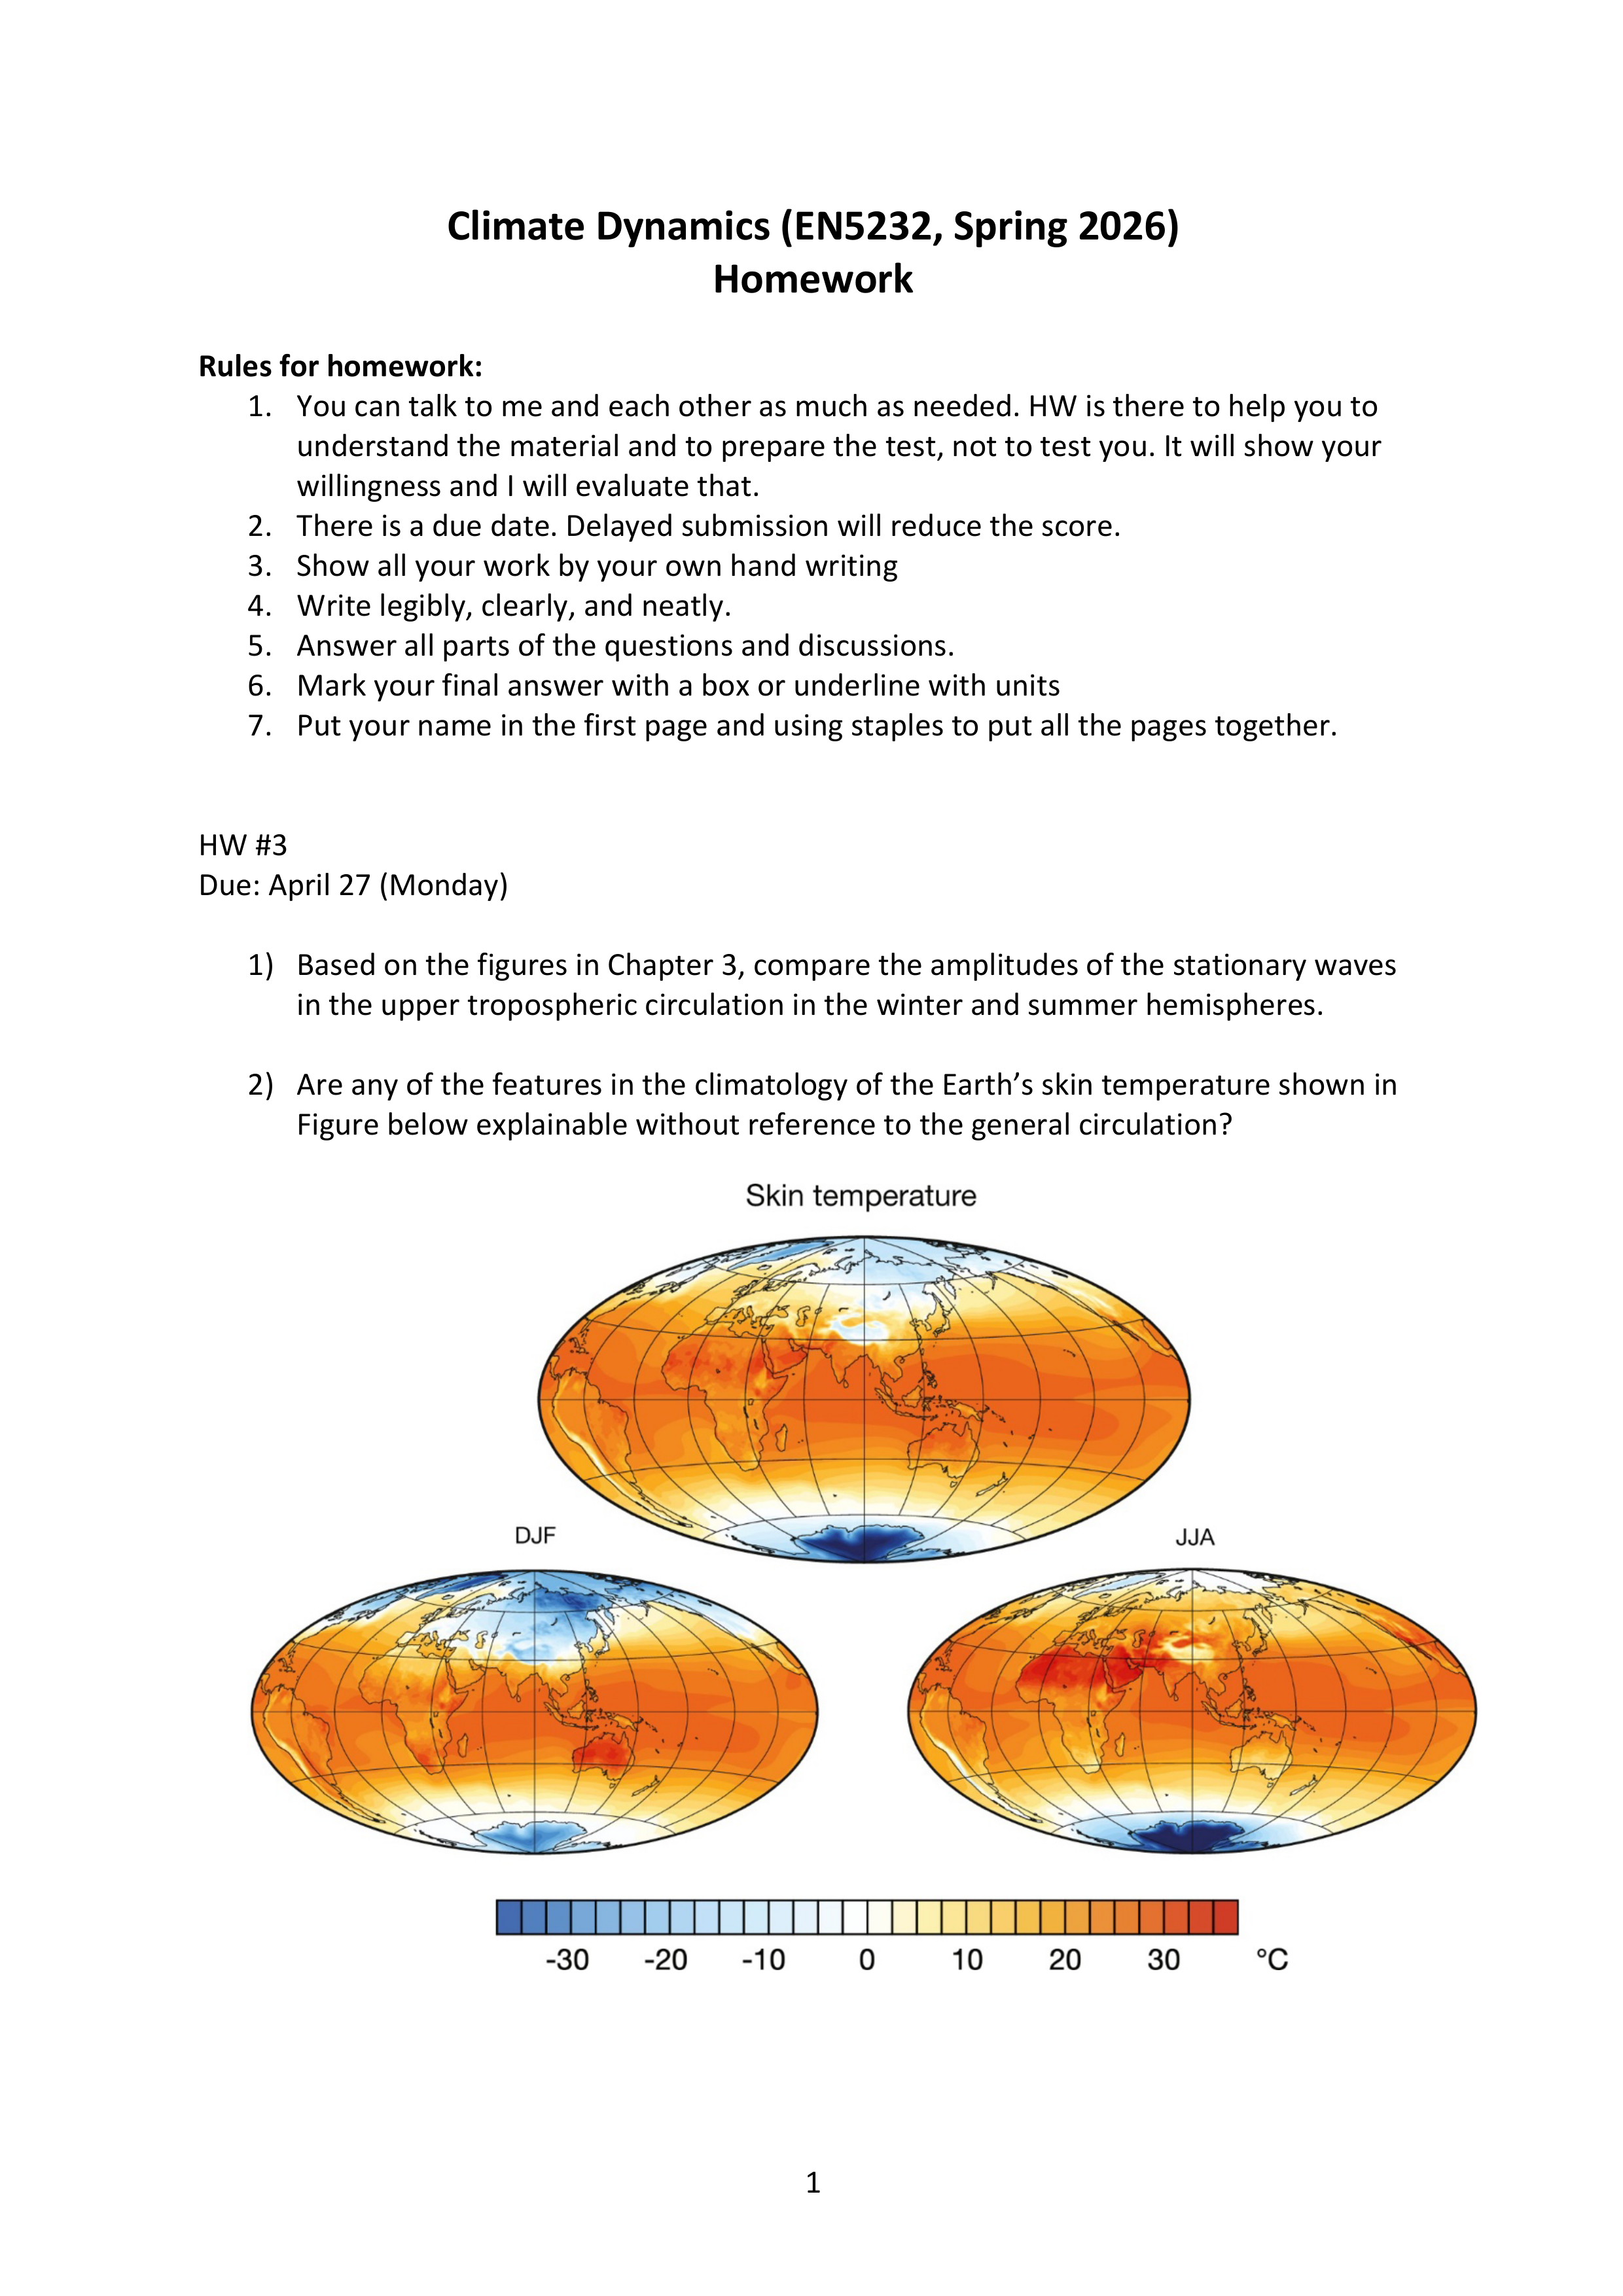
\includegraphics[width=0.85\textwidth]{images/ch03/hw3_skin_temp.png}
  \caption{Climatological skin temperature ($^{\circ}$C) for DJF (top) and JJA (bottom).
           \hisu{DJF: 시베리아/캐나다 $<$$-30^{\circ}$C (극한 대륙 냉각), 열대 및 SH 대륙 따뜻함;
                  JJA: 사하라/아라비아 반도 $>$$40^{\circ}$C, 북반구 대륙 전반 고온, 남극대 극저온}}
  \label{fig:ch03-skin-temp}
\end{figure}

\subsection{Features Explainable Without the General Circulation}

지표 온도 분포의 일부 특징은 대기 대순환(general circulation)을 고려하지 않고도
\textgr{복사 균형}과 \textgr{지표 물성 차이}만으로 설명할 수 있다.

\begin{definition}[Radiative Equilibrium Surface Temperature]
대기 순환이 전혀 없는 경우, 지표 온도는 local radiative balance에 의해 결정된다.
입사 태양 복사 $F(\phi) = \frac{S_{0}}{\pi}\cos\phi$ (연평균, axial tilt 무시)와
단일 슬래브 대기의 온실 효과를 고려하면:
\begin{equation}
  T_{s}(\phi) \propto \cos^{1/4}\phi,
  \label{eq:rad-equil-Ts}
\end{equation}
이는 적도에서 극으로 갈수록 온도가 감소하는 1차 근사를 제공한다.
\end{definition}

\begin{remark}[General circulation 없이 설명 가능한 특징]
\begin{enumerate}
  \item \textgr{Equator-to-pole temperature gradient}: 태양 복사의 위도별 분포
        ($\propto \cos\phi$ geometry)에 의해 저위도가 따뜻하고 고위도가 차가운 기본 구조가 설명된다.
  \item \textgr{Seasonal cycle}: 지구 자전축의 기울기 ($23.4^{\circ}$)에 의해 여름 반구가
        더 많은 일사를 받아 따뜻해지고, 겨울 반구가 차가워지는 패턴이 나타난다.
  \item \textgr{Land--sea contrast (thermal inertia)}: 대륙은 열용량이 작아 계절에 대해
        빠르게 반응하는 반면, 해양은 열용량이 커서 계절 변동이 작다.
        \begin{itemize}
          \item DJF에 시베리아/캐나다 내륙이 극도로 차가운 것 ($<$$-30^{\circ}$C)
          \item JJA에 사하라/아라비아 반도가 $>$$40^{\circ}$C로 매우 뜨거운 것
          \item 같은 위도에서 해양 표면 온도의 계절 변동이 대륙보다 작은 것
        \end{itemize}
  \item \textgr{High albedo at high latitudes}: 빙하/설빙 지역의 높은 알베도가 극지방의
        추가적 냉각에 기여한다 (ice--albedo feedback).
\end{enumerate}
\end{remark}

\begin{hisublock}
``대순환 없이 설명 가능''이란 = 태양 복사의 위도 분포, 계절 변동, 지표 물성 차이만으로
설명된다는 의미이다.  이 요인들은 purely local/radiative한 것들이다.
\end{hisublock}

\subsection{Features Requiring the General Circulation}

\begin{remark}[General circulation이 필요한 특징]
반면, 다음 특징들은 대기 및 해양 순환을 고려하지 않으면 설명할 수 없다:
\begin{enumerate}
  \item \textgr{관측된 적도--극 온도 경도가 복사 평형보다 훨씬 작다}:
        복사 평형만으로는 적도--극 온도 차이가 $\sim$100\,K 이상이어야 하지만,
        관측에서는 $\sim$50--60\,K 수준이다.
        이 차이의 원인은 대기와 해양에 의한 \textgr{poleward heat transport}이다.
  \item \textgr{서안 경계류에 의한 고위도 온난화}:
        Gulf Stream과 Kuroshio가 저위도의 따뜻한 물을 고위도로 수송하여
        서유럽과 동아시아 해안의 기온을 같은 위도의 대륙 내부보다 현저히 높인다.
        예: 노르웨이 해안이 같은 위도의 시베리아보다 20--30\,K 이상 따뜻하다.
  \item \textgr{동안 용승대 (eastern boundary upwelling)에 의한 아열대 해안 냉각}:
        무역풍에 의한 offshore Ekman transport가 차가운 심층수의 용승을 유발하여,
        캘리포니아/페루/서아프리카 해안의 SST (따라서 skin temperature)를
        같은 위도의 서태평양보다 훨씬 차갑게 만든다.
  \item \textgr{아열대 사막 분포}: Hadley cell의 하강 지역 ($\sim$$30^{\circ}$\,N/S)에서
        맑은 하늘과 건조한 공기가 지표 가열을 극대화하여, 사하라/아라비아/호주 내륙의
        극단적 고온을 유발한다.  이것은 단순히 위도에 의한 일사량만으로는 설명할 수 없다.
  \item \textgr{적도 태평양의 동서 비대칭}: 적도에서도 skin temperature가 동서로 균일하지 않다.
        서태평양 warm pool ($>$$28^{\circ}$C)과 동태평양 cold tongue ($\sim$22--24$^{\circ}$C)의 대비는
        Walker circulation과 equatorial upwelling에 의해 유지된다.
\end{enumerate}
\end{remark}

\begin{hisublock}
핵심 결론: skin temperature의 \textbf{1차적 패턴} (적도--극 경도, 계절 변동, 대륙--해양 대비)은
복사와 열용량만으로 설명 가능하지만, \textbf{세부 구조와 크기}
(실제 적도--극 차이 축소, 서안 난류에 의한 고위도 온난화, 동안 용승에 의한 냉각,
아열대 사막 고온, 적도 동서 비대칭)는 대기--해양 순환이 반드시 필요하다.
\end{hisublock}

\begin{hisublock}
\textbf{참고 문헌 가이드:}
\begin{itemize}
  \item Marshall and Plumb (2008), \textit{Atmosphere, Ocean and Climate Dynamics}, Ch.5.1--5.3 (pp.62--73, PDF pp.83--94) -- 복사 평형 온도와 관측 온도의 비교, poleward heat transport의 필요성
  \item Hartmann (1994), \textit{Global Physical Climatology}, Ch.1 (pp.1--20) -- 전구 평균 지표 온도 ($\sim$288\,K)와 위도별 분포 개관
  \item Peixoto and Oort (1992), \textit{Physics of Climate}, Ch.7.2 (pp.137--143) -- 지표/대기 온도의 관측 분포
\end{itemize}
\end{hisublock}


\vspace{12pt}
\begin{highlight}
\textgr{Chapter Summary.}
관측된 atmospheric general circulation은 다음과 같은 특징을 갖는다:
(1)~thermally driven overturning cells (Hadley, Ferrel, polar);
(2)~thermal wind relationship에 의해 유지되는 subtropical jet streams;
(3)~특히 NH에서 zonal symmetry를 깨뜨리는 강한 land--sea contrast;
(4)~solar heating maximum의 이동에 의해 구동되는 극적인 seasonal variation;
(5)~SST, precipitation, large-scale wind field 사이의 긴밀한 coupling.
이러한 관측은 이후 장에서 전개되는 dynamical theory의 동기를 제공한다.
\end{highlight}
